\documentclass[10pt]{article}

\usepackage[margin=0.9in]{geometry}
\usepackage{times}
\usepackage{microtype}
\usepackage{amsmath,amssymb,amsfonts}
\usepackage{booktabs}
\usepackage{graphicx}
\usepackage{subcaption}
\usepackage{multirow}
\usepackage{xcolor}
\usepackage{enumitem}
\usepackage{algorithm}
\usepackage{algpseudocode}
\usepackage[numbers,sort&compress]{natbib}
\usepackage[colorlinks=true,linkcolor=blue,citecolor=blue,urlcolor=blue]{hyperref}

\graphicspath{{figures/}}
\setlength{\textfloatsep}{8pt plus 2pt minus 2pt}
\setlength{\floatsep}{8pt plus 2pt minus 2pt}
\setlength{\intextsep}{8pt plus 2pt minus 2pt}
\setlist[itemize]{leftmargin=*,topsep=2pt,itemsep=1pt}

\title{\vspace{-1.0em}
CS-WAE: Class-Structured Spherical Cauchy Wasserstein Auto-Encoders
for Label-Guided Generative Clustering
\vspace{-0.2em}}

\author{
Anonymous Authors\\
\small Anonymous Institution\\
\small \texttt{anonymous@example.com}
}

\date{}

\begin{document}
\maketitle

\begin{abstract}
Learning a latent space that is simultaneously useful for clustering, reconstruction, and sampling remains difficult for auto-encoding generative models. Standard variational auto-encoders use Euclidean Gaussian latents, while Wasserstein auto-encoders align the aggregated posterior with a prior but do not by themselves impose class-level organization. We introduce CS-WAE, a class-structured spherical Cauchy Wasserstein auto-encoder that places representations on a hypersphere and aligns them with learnable class priors through a dual maximum mean discrepancy objective. The model uses a Spherical Cauchy reparameterization based on Mobius transformations, a reconstruction objective combining pixel and perceptual losses, and two complementary regularizers: a label-guided MMD term that aligns each class with its corresponding spherical prior, and an unsupervised MMD term that preserves global prior matching. Across MNIST and Fashion-MNIST, CS-WAE obtains strong clustering performance while retaining competitive generation quality. On MNIST, it reaches $92.9{\pm}3.9\%$ clustering accuracy over three seeds; on Fashion-MNIST, it reaches $79.0{\pm}8.0\%$. Against VAE, VaDE, and WAE-MMD baselines under a 50-epoch protocol, CS-WAE improves clustering accuracy by roughly 26--34 percentage points. Ablations show that removing supervised MMD, replacing the hypersphere with a Euclidean latent space, or replacing the Spherical Cauchy prior with a von Mises--Fisher prior substantially degrades clustering or sampling. These results support a simple thesis: for label-guided generative clustering, the geometry of the latent space and the distributional alignment objective must be designed together.
\end{abstract}

\section{Introduction}

Auto-encoding generative models are attractive because they combine representation learning with reconstruction and sampling. In practice, however, the same latent space rarely serves all downstream purposes equally well. A latent representation may reconstruct accurately while failing to form useful clusters; conversely, a clustering-friendly representation may become difficult to sample from. This tension is especially visible in variational auto-encoders (VAEs) \citep{kingma2013autoencoding} and Wasserstein auto-encoders (WAEs) \citep{tolstikhin2017wasserstein}: both provide principled generative frameworks, but neither automatically enforces class-separated geometry in the learned representation.

Deep generative clustering methods, such as VaDE \citep{jiang2016variational}, address this issue by introducing mixture structure in the latent prior. Yet Gaussian mixture priors remain Euclidean and unbounded. For visual categories whose identities are better represented by directions than by radii, hyperspherical latent spaces are a natural alternative. Hyperspherical VAEs \citep{davidson2018hyperspherical} replace Gaussian latents with distributions on the unit sphere, commonly the von Mises--Fisher (vMF) distribution. Recent Spherical Cauchy VAEs \citep{sablica2025hyperspherical} further show that heavy-tailed distributions on the sphere can provide efficient Mobius-transform reparameterization and avoid some numerical difficulties of vMF distributions.

This paper studies a related but distinct question: can a spherical heavy-tailed latent distribution be combined with WAE-style distribution matching to obtain a representation that is both class-structured and generative? We propose CS-WAE, a class-structured Spherical Cauchy Wasserstein auto-encoder. The model maps each input image to parameters of a Spherical Cauchy distribution on $\mathbb{S}^{d-1}$, samples latents via a Mobius reparameterization, and decodes them with a convolutional decoder. Its prior consists of $K$ learnable class centers on the sphere. Training uses a reconstruction loss and a dual MMD regularizer: a supervised, per-class MMD term that aligns samples from class $c$ with the $c$-th class prior, and an unsupervised aggregated MMD term that aligns the full encoded distribution with a mixture over all class priors.

\paragraph{Scope.}
CS-WAE is not an unsupervised clustering model in the strict sense, because labels are used during training through the supervised MMD term. We therefore frame the method as \emph{label-guided generative clustering}: the model learns a latent geometry whose clusters correspond to known class labels during training, while evaluation uses K-means and Hungarian matching on latent representations. This positioning is important both technically and scientifically. It allows us to test whether explicit class-prior matching improves the latent geometry beyond reconstruction alone, without overstating the method as label-free clustering.

\paragraph{Contributions.}
The main contributions are:
\begin{itemize}
    \item We introduce a WAE-style auto-encoder with Spherical Cauchy latent variables and learnable class priors on $\mathbb{S}^{d-1}$.
    \item We propose a dual MMD objective combining per-class supervised alignment with global aggregated-posterior matching.
    \item We provide a controlled empirical study on MNIST and Fashion-MNIST, including multi-seed CS-WAE runs, baseline comparisons against VAE, VaDE, and WAE-MMD, and ablations of supervised MMD, spherical geometry, and the Spherical Cauchy prior.
    \item We show that CS-WAE substantially improves clustering accuracy over the considered baselines, while exposing clear trade-offs between reconstruction quality, sampling quality, and latent class structure.
\end{itemize}

\paragraph{Paper organization.}
Section~2 reviews the lines of work that motivate CS-WAE: auto-encoding generative models, deep clustering, hyperspherical latent variables, and distribution matching. Section~3 presents the model and training objective. Section~4 gives the experimental protocol and quantitative results. Section~5 discusses why the components interact as they do, what claims are supported by the evidence, and what remains incomplete. Appendix sections give additional reproducibility details and recommended next experiments.

\section{Related Work}

\paragraph{Variational and Wasserstein auto-encoders.}
VAEs \citep{kingma2013autoencoding} optimize an evidence lower bound using amortized inference and a reparameterization trick. While successful, the KL regularizer can encourage posterior collapse or overly simple latent structure. WAEs \citep{tolstikhin2017wasserstein} instead match the aggregated posterior to a prior, often using MMD or adversarial penalties, and can produce stable generative models with improved sample quality. Sliced-Wasserstein auto-encoders \citep{kolouri2018sliced} further simplify distribution matching using one-dimensional projections. CS-WAE follows the WAE principle of matching an encoded distribution to a samplable prior, but moves this matching to a class-structured hyperspherical prior.

\paragraph{Deep generative clustering.}
Deep Embedded Clustering (DEC) \citep{xie2015unsupervised} learns representations by optimizing a clustering objective in a learned feature space. VaDE \citep{jiang2016variational} integrates a Gaussian mixture prior into a VAE and provides a generative clustering model. These methods are important references because they connect latent generative modeling to cluster discovery. Our work differs in two ways. First, we use class labels during training to supervise prior alignment, so our setting is label-guided rather than fully unsupervised. Second, we impose hyperspherical geometry with heavy-tailed class priors, instead of a Euclidean Gaussian mixture.

\paragraph{Hyperspherical latent variables.}
Hyperspherical VAEs \citep{davidson2018hyperspherical} motivate vMF latent distributions when directional geometry is more appropriate than Euclidean geometry. Spherical sliced-Wasserstein distances \citep{bonet2022spherical} show that optimal-transport-inspired discrepancies can be adapted to spherical spaces. Recent work on Spherical Cauchy VAEs \citep{sablica2025hyperspherical} argues that Spherical Cauchy distributions provide efficient reparameterization and practical stability. CS-WAE builds on this motivation, but uses Spherical Cauchy variables in a WAE-like distribution matching framework with class-specific priors.

\paragraph{Evaluation metrics.}
We evaluate clustering using K-means followed by Hungarian assignment, reporting ACC, normalized mutual information (NMI), and adjusted Rand index (ARI). Generation quality is measured by Fr\'echet Inception Distance (FID) \citep{heusel2017gans}. Reconstruction quality is measured using SSIM, PSNR, and LPIPS \citep{zhang2018unreasonable}. The inclusion of both clustering and generative metrics is essential: a model can reconstruct well while sampling poorly, as our WAE-MMD baseline demonstrates.

\paragraph{Positioning relative to prior work.}
The closest conceptual relatives are WAE-MMD, VaDE, hyperspherical VAEs, and Spherical Cauchy VAEs. WAE-MMD supplies the aggregated-posterior matching viewpoint, but uses a Euclidean latent prior and does not impose class structure. VaDE supplies a generative clustering baseline, but its mixture prior is Gaussian and its latent geometry is not constrained to the sphere. Hyperspherical VAEs motivate directional latents, but most implementations rely on vMF variables and an ELBO objective. Spherical Cauchy VAEs motivate a practical heavy-tailed distribution on the sphere, but do not study class-specific WAE-style MMD alignment. CS-WAE occupies the intersection of these ideas: it is a WAE-like objective, uses a Spherical Cauchy latent family, and learns class-indexed priors on the hypersphere.

\section{Method}

\subsection{Problem Setting}

Let $\mathcal{D}=\{(x_i,y_i)\}_{i=1}^{n}$ be a labeled image dataset with $K$ classes, where $x_i\in[0,1]^{1\times 28\times 28}$ and $y_i\in\{1,\dots,K\}$. We seek an encoder-decoder model that learns a latent representation $z\in\mathbb{S}^{d-1}$ useful for three purposes: reconstruction of $x$, class-structured clustering, and sampling from a prior. In the experiments, $d=32$ and $K=10$.

\subsection{Design Goals}

The architecture is built around three design goals.
First, the latent space should make class identity geometrically visible. A simple K-means classifier should not need a deep nonlinear head to recover labels from the learned representation. This motivates a class-structured prior instead of a single isotropic prior.
Second, the prior must remain generative. If the decoder is only trained on encoded points and not on samples from the intended prior, generated images can be poor even when reconstructions are accurate. This motivates aggregated-posterior matching rather than a purely discriminative clustering loss.
Third, the latent geometry should match the intended representation. Euclidean latents allow the encoder to use radius as an uncontrolled degree of freedom; a hypersphere forces information into direction and makes class centers comparable by angular separation.

These goals lead to a simple principle: class structure should be imposed at the level of distributions on the sphere, not merely through pointwise classification. CS-WAE therefore does not add a cross-entropy classifier to the latent vector. Instead, it aligns the empirical latent distribution of each class with a corresponding samplable prior distribution. This choice keeps the model generative: at test time, samples can be drawn directly from class priors and decoded.

\subsection{Spherical Cauchy Encoder and Decoder}

The encoder $E_\phi$ maps an image $x$ to two quantities:
\begin{equation}
    (\tilde{\mu}_q, s_q) = E_\phi(x), \qquad
    \mu_q = \frac{\tilde{\mu}_q}{\|\tilde{\mu}_q\|_2}, \qquad
    \rho_q = \sigma(s_q)(1-\epsilon),
\end{equation}
where $\mu_q\in\mathbb{S}^{d-1}$ is a direction and $\rho_q\in(0,1)$ is a concentration-like scalar. A latent sample is generated through a Mobius reparameterization
\begin{equation}
    \epsilon_s \sim \mathrm{Unif}(\mathbb{S}^{d-1}), \qquad
    z_q = T_{\mu_q,\rho_q}(\epsilon_s),
\end{equation}
where $T$ denotes the Spherical Cauchy Mobius transform. The decoder $D_\theta$ maps $z_q$ back to an image $\hat{x}=D_\theta(z_q)$. In implementation, both encoder and decoder are compact convolutional networks.

The deterministic direction $\mu_q$ is also used as the representation for clustering evaluation. This mirrors the common VAE practice of evaluating the posterior mean rather than noisy samples. The stochastic sample $z_q$ is used for training the decoder and matching the posterior to the prior. Separating these roles reduces evaluation noise while retaining a stochastic generative training path.

\subsection{Class-Structured Spherical Prior}

CS-WAE uses $K$ learnable prior directions
\begin{equation}
    M = \{m_1,\dots,m_K\}, \qquad m_c \in \mathbb{S}^{d-1}.
\end{equation}
Each class prior is a Spherical Cauchy distribution centered at $m_c$ with fixed prior radius $\rho_p=0.7$. To sample from class $c$,
\begin{equation}
    \epsilon_s \sim \mathrm{Unif}(\mathbb{S}^{d-1}), \qquad
    z_p^{(c)} = T_{m_c,\rho_p}(\epsilon_s).
\end{equation}
The class priors are normalized during loss computation, so their effective support remains on the sphere.

The prior centers are learnable rather than fixed vertices of a simplex. A fixed spherical code would impose equal angular distances between all classes, which may not reflect visual similarity. For example, Fashion-MNIST contains several clothing categories that are naturally closer to one another than to footwear or bags. Learnable priors allow the model to discover an arrangement that balances separability with reconstruction and sampling. The supervised MMD term prevents this flexibility from degenerating into arbitrary class mixing.

\subsection{Dual MMD Objective}

Maximum mean discrepancy (MMD) \citep{gretton2012kernel} compares distributions through kernel mean embeddings. Given samples $A=\{a_i\}_{i=1}^{n}$ and $B=\{b_j\}_{j=1}^{m}$, the squared empirical MMD is
\begin{align}
    \widehat{\mathrm{MMD}}^2(A,B)
    &= \frac{1}{n^2}\sum_{i,i'} k(a_i,a_{i'})
    + \frac{1}{m^2}\sum_{j,j'} k(b_j,b_{j'})
    - \frac{2}{nm}\sum_{i,j} k(a_i,b_j).
\end{align}

CS-WAE uses two MMD terms. The supervised term aligns each class-conditional encoded distribution to its corresponding class prior:
\begin{equation}
    \mathcal{L}_{\mathrm{sup}}
    =
    \frac{1}{K}\sum_{c=1}^{K}
    \mathrm{MMD}\left(
        \{z_q^i: y_i=c\},
        \{z_p^{(c),j}\}_{j=1}^{n_c}
    \right).
\end{equation}
The unsupervised aggregated term aligns the full encoded distribution with samples from the mixture over class priors:
\begin{equation}
    \mathcal{L}_{\mathrm{unsup}}
    =
    \mathrm{MMD}\left(
        \{z_q^i\}_{i=1}^{b},
        \{z_p^{(r_j),j}: r_j\sim\mathrm{Unif}(\{1,\dots,K\})\}_{j=1}^{b}
    \right).
\end{equation}
The supervised term creates class separation; the unsupervised term preserves global sampleability from the prior mixture.

Both terms are necessary for different reasons. The supervised MMD term is class-aware but local: it compares class-conditional batches against their corresponding priors. The unsupervised MMD term is class-agnostic but global: it checks whether the entire encoded batch resembles samples from the prior mixture. Without the supervised term, the model can match a mixture distribution while failing to preserve class identity. Without the unsupervised term, class priors can become useful anchors but may not collectively approximate a well-sampled generative prior.

\subsection{Why Spherical Cauchy?}

The Spherical Cauchy distribution is useful here because it combines spherical support with heavy-tailed behavior and a reparameterization based on Mobius transformations. In a class-structured latent space, overly concentrated priors can make each class region brittle: samples close to the center reconstruct well, but off-center samples may decode poorly or collapse into ambiguous images. A heavier-tailed spherical distribution allows each class prior to cover a broader region of the sphere while still maintaining a center. This is particularly attractive for classes with large intra-class variability.

The comparison with vMF priors in the ablation study is therefore not only a distributional substitution; it tests whether a different concentration geometry changes the representation-generation trade-off. Empirically, vMF behaves inconsistently across the two datasets. On MNIST it gives high reconstruction scores in the old ablation run but poor clustering. On Fashion-MNIST it partially preserves clustering but severely harms sample quality. The Spherical Cauchy prior gives the most consistent compromise under the current protocol.

\subsection{Training Objective}

The reconstruction loss combines binary cross-entropy and LPIPS:
\begin{equation}
    \mathcal{L}_{\mathrm{rec}}
    =
    \lambda_{\mathrm{BCE}}\mathrm{BCE}(x,\hat{x})
    +
    \lambda_{\mathrm{LPIPS}}\mathrm{LPIPS}(x,\hat{x}),
\end{equation}
with $\lambda_{\mathrm{BCE}}=0.3$ and $\lambda_{\mathrm{LPIPS}}=0.7$. The total objective is
\begin{equation}
    \mathcal{L}
    =
    \mathcal{L}_{\mathrm{rec}}
    +
    \alpha(t)\mathcal{L}_{\mathrm{sup}}
    +
    \beta(t)\mathcal{L}_{\mathrm{unsup}},
\end{equation}
where $\alpha(t)$ and $\beta(t)$ are linearly annealed over the first 20 epochs to final weights 20 and 50, respectively. We use Adam with learning rate $10^{-3}$, batch size 128, gradient clipping at norm 1.0, and StepLR with step 30 and decay 0.5.

\begin{algorithm}[t]
\caption{CS-WAE training step}
\label{alg:training}
\begin{algorithmic}[1]
\Require Mini-batch $(x,y)$, encoder $E_\phi$, decoder $D_\theta$, class prior centers $\{m_c\}_{c=1}^{K}$
\State Encode $(\tilde{\mu}_q,s_q)\leftarrow E_\phi(x)$
\State Normalize $\mu_q\leftarrow \tilde{\mu}_q/\|\tilde{\mu}_q\|_2$ and compute $\rho_q\leftarrow \sigma(s_q)(1-\epsilon)$
\State Sample $\epsilon_s\sim\mathrm{Unif}(\mathbb{S}^{d-1})$ and compute $z_q\leftarrow T_{\mu_q,\rho_q}(\epsilon_s)$
\State Decode $\hat{x}\leftarrow D_\theta(z_q)$
\State Compute $\mathcal{L}_{\mathrm{rec}}$ from BCE and LPIPS
\For{class $c=1,\dots,K$}
    \State Sample $z_p^{(c)}$ from the Spherical Cauchy prior centered at normalized $m_c$
    \State Accumulate class-conditional MMD between $\{z_q^i:y_i=c\}$ and $z_p^{(c)}$
\EndFor
\State Sample prior mixture latents by drawing random class indices $r_j\sim\mathrm{Unif}(\{1,\dots,K\})$
\State Compute $\mathcal{L}_{\mathrm{sup}}$, $\mathcal{L}_{\mathrm{unsup}}$, and total loss $\mathcal{L}$
\State Update $\phi,\theta,\{m_c\}$ using Adam
\end{algorithmic}
\end{algorithm}

Algorithm~\ref{alg:training} summarizes one training step. The class prior centers are optimized jointly with the encoder and decoder. During generation, the encoder is not used: a class index is sampled or specified, a latent is sampled from the corresponding Spherical Cauchy prior, and the decoder maps it to image space.

\section{Experiments}

\subsection{Datasets and Protocol}

We evaluate on MNIST \citep{lecun1998gradient} and Fashion-MNIST \citep{xiao2017fashion}. Both contain $28\times 28$ grayscale images and 10 classes, but Fashion-MNIST is visually more ambiguous and therefore a stronger test of latent class structure. Each main CS-WAE result is reported over three seeds $\{0,1,2\}$ for 50 epochs. Baseline comparisons and ablations are currently reported with seed 0 for 50 epochs. This asymmetry is a limitation; we report it explicitly rather than hiding it.

The evaluated baselines are VAE, WAE-MMD, VaDE, and CS-WAE under the same epoch budget. For clustering, we extract latent representations on the test set, run K-means with $K=10$, and align cluster IDs to labels using the Hungarian algorithm. We report ACC, NMI, and ARI. For generation, we sample 10,000 generated images and compare them to 10,000 real test images using FID. Reconstruction metrics include SSIM, PSNR, and LPIPS; the main paper emphasizes clustering and FID for compactness.

\subsection{Main Multi-Seed Results}

\begin{table}[t]
\centering
\caption{Main CS-WAE results over three seeds and 50 epochs. ACC, NMI, and ARI are percentages.}
\label{tab:main}
\begin{tabular}{lcccc}
\toprule
Dataset & ACC$\uparrow$ & NMI$\uparrow$ & ARI$\uparrow$ & FID$\downarrow$ \\
\midrule
MNIST & $92.9 \pm 3.9$ & $89.0 \pm 0.8$ & $88.5 \pm 3.2$ & $19.4 \pm 5.3$ \\
Fashion-MNIST & $79.0 \pm 8.0$ & $76.2 \pm 1.4$ & $69.0 \pm 6.1$ & $50.7 \pm 1.6$ \\
\bottomrule
\end{tabular}
\end{table}

Table~\ref{tab:main} summarizes the main result. CS-WAE obtains high clustering accuracy on MNIST and remains strong on Fashion-MNIST, despite the latter's more confusable categories. The standard deviation in ACC is non-negligible, especially on Fashion-MNIST. This indicates that the method is sensitive to initialization, and that reporting a single best seed would overstate stability. NMI varies less than ACC, suggesting that the learned latent structure is often meaningful even when the exact K-means assignment varies.

\begin{table}[t]
\centering
\caption{Per-seed CS-WAE results. ACC, NMI, and ARI are percentages. Seed-level reporting is important because clustering accuracy varies more than NMI and reconstruction metrics.}
\label{tab:perseed}
\resizebox{\linewidth}{!}{
\begin{tabular}{llccccccc}
\toprule
Dataset & Seed & ACC$\uparrow$ & NMI$\uparrow$ & ARI$\uparrow$ & FID$\downarrow$ & SSIM$\uparrow$ & LPIPS$\downarrow$ & PSNR$\uparrow$ \\
\midrule
\multirow{3}{*}{MNIST}
& 0 & 87.35 & 88.63 & 84.11 & 26.95 & 0.813 & 0.060 & 16.38 \\
& 1 & 95.28 & 88.23 & 89.88 & 15.48 & 0.861 & 0.049 & 17.77 \\
& 2 & 96.10 & 90.08 & 91.62 & 15.82 & 0.878 & 0.044 & 18.36 \\
\midrule
\multirow{3}{*}{Fashion-MNIST}
& 0 & 82.24 & 77.37 & 72.07 & 49.89 & 0.697 & 0.120 & 16.51 \\
& 1 & 68.03 & 74.20 & 60.53 & 52.82 & 0.678 & 0.126 & 16.20 \\
& 2 & 86.67 & 76.91 & 74.50 & 49.26 & 0.689 & 0.121 & 16.36 \\
\bottomrule
\end{tabular}}
\end{table}

Table~\ref{tab:perseed} makes the seed dependence explicit. On MNIST, seed 0 has substantially worse FID and ACC than seeds 1 and 2, even though its NMI remains close to the others. On Fashion-MNIST, seed 1 is the clustering outlier, with ACC dropping to 68.03 while FID changes only mildly. This suggests two distinct stability regimes: the decoder's sample distribution can be relatively stable while the exact cluster-label alignment remains sensitive. For a paper submission, this makes mean--standard deviation reporting mandatory, and it motivates future work on either more seeds or a more stable clustering head.

\subsection{Baseline Comparison}

\begin{table}[t]
\centering
\caption{Baseline comparison at seed 0 and 50 epochs. ACC, NMI, and ARI are percentages.}
\label{tab:baselines}
\resizebox{\linewidth}{!}{
\begin{tabular}{llcccc}
\toprule
Dataset & Method & ACC$\uparrow$ & NMI$\uparrow$ & ARI$\uparrow$ & FID$\downarrow$ \\
\midrule
\multirow{4}{*}{MNIST}
& CS-WAE & \textbf{86.9} & \textbf{85.0} & \textbf{82.1} & \textbf{15.2} \\
& VAE & 60.9 & 55.3 & 45.6 & 18.8 \\
& VaDE & 57.8 & 53.4 & 42.4 & 17.4 \\
& WAE-MMD & 57.5 & 50.6 & 38.7 & 138.3 \\
\midrule
\multirow{4}{*}{Fashion-MNIST}
& CS-WAE & \textbf{84.8} & \textbf{75.2} & \textbf{71.9} & 54.2 \\
& VAE & 53.6 & 49.7 & 37.1 & 52.1 \\
& VaDE & 50.3 & 50.7 & 36.3 & \textbf{48.7} \\
& WAE-MMD & 53.9 & 57.5 & 41.2 & 239.6 \\
\bottomrule
\end{tabular}}
\end{table}

Table~\ref{tab:baselines} shows that CS-WAE improves clustering accuracy by approximately 26--29 percentage points on MNIST and 31--34 points on Fashion-MNIST relative to the evaluated baselines. The result is strongest for clustering metrics. FID is best on MNIST, but on Fashion-MNIST VaDE obtains a lower FID while clustering much worse. This distinction matters: CS-WAE should not be described as uniformly best on every generative metric. Its central advantage is the combination of strong class-structured latent geometry with competitive sampling.

WAE-MMD highlights the difference between reconstruction and generation. It obtains high reconstruction quality in the full logs, yet its FID is poor on both datasets. This suggests that matching a simple Euclidean prior can be insufficient for sampling even when the auto-encoder reconstructs well. CS-WAE's class-structured spherical prior reduces this mismatch.

\begin{figure}[t]
\centering
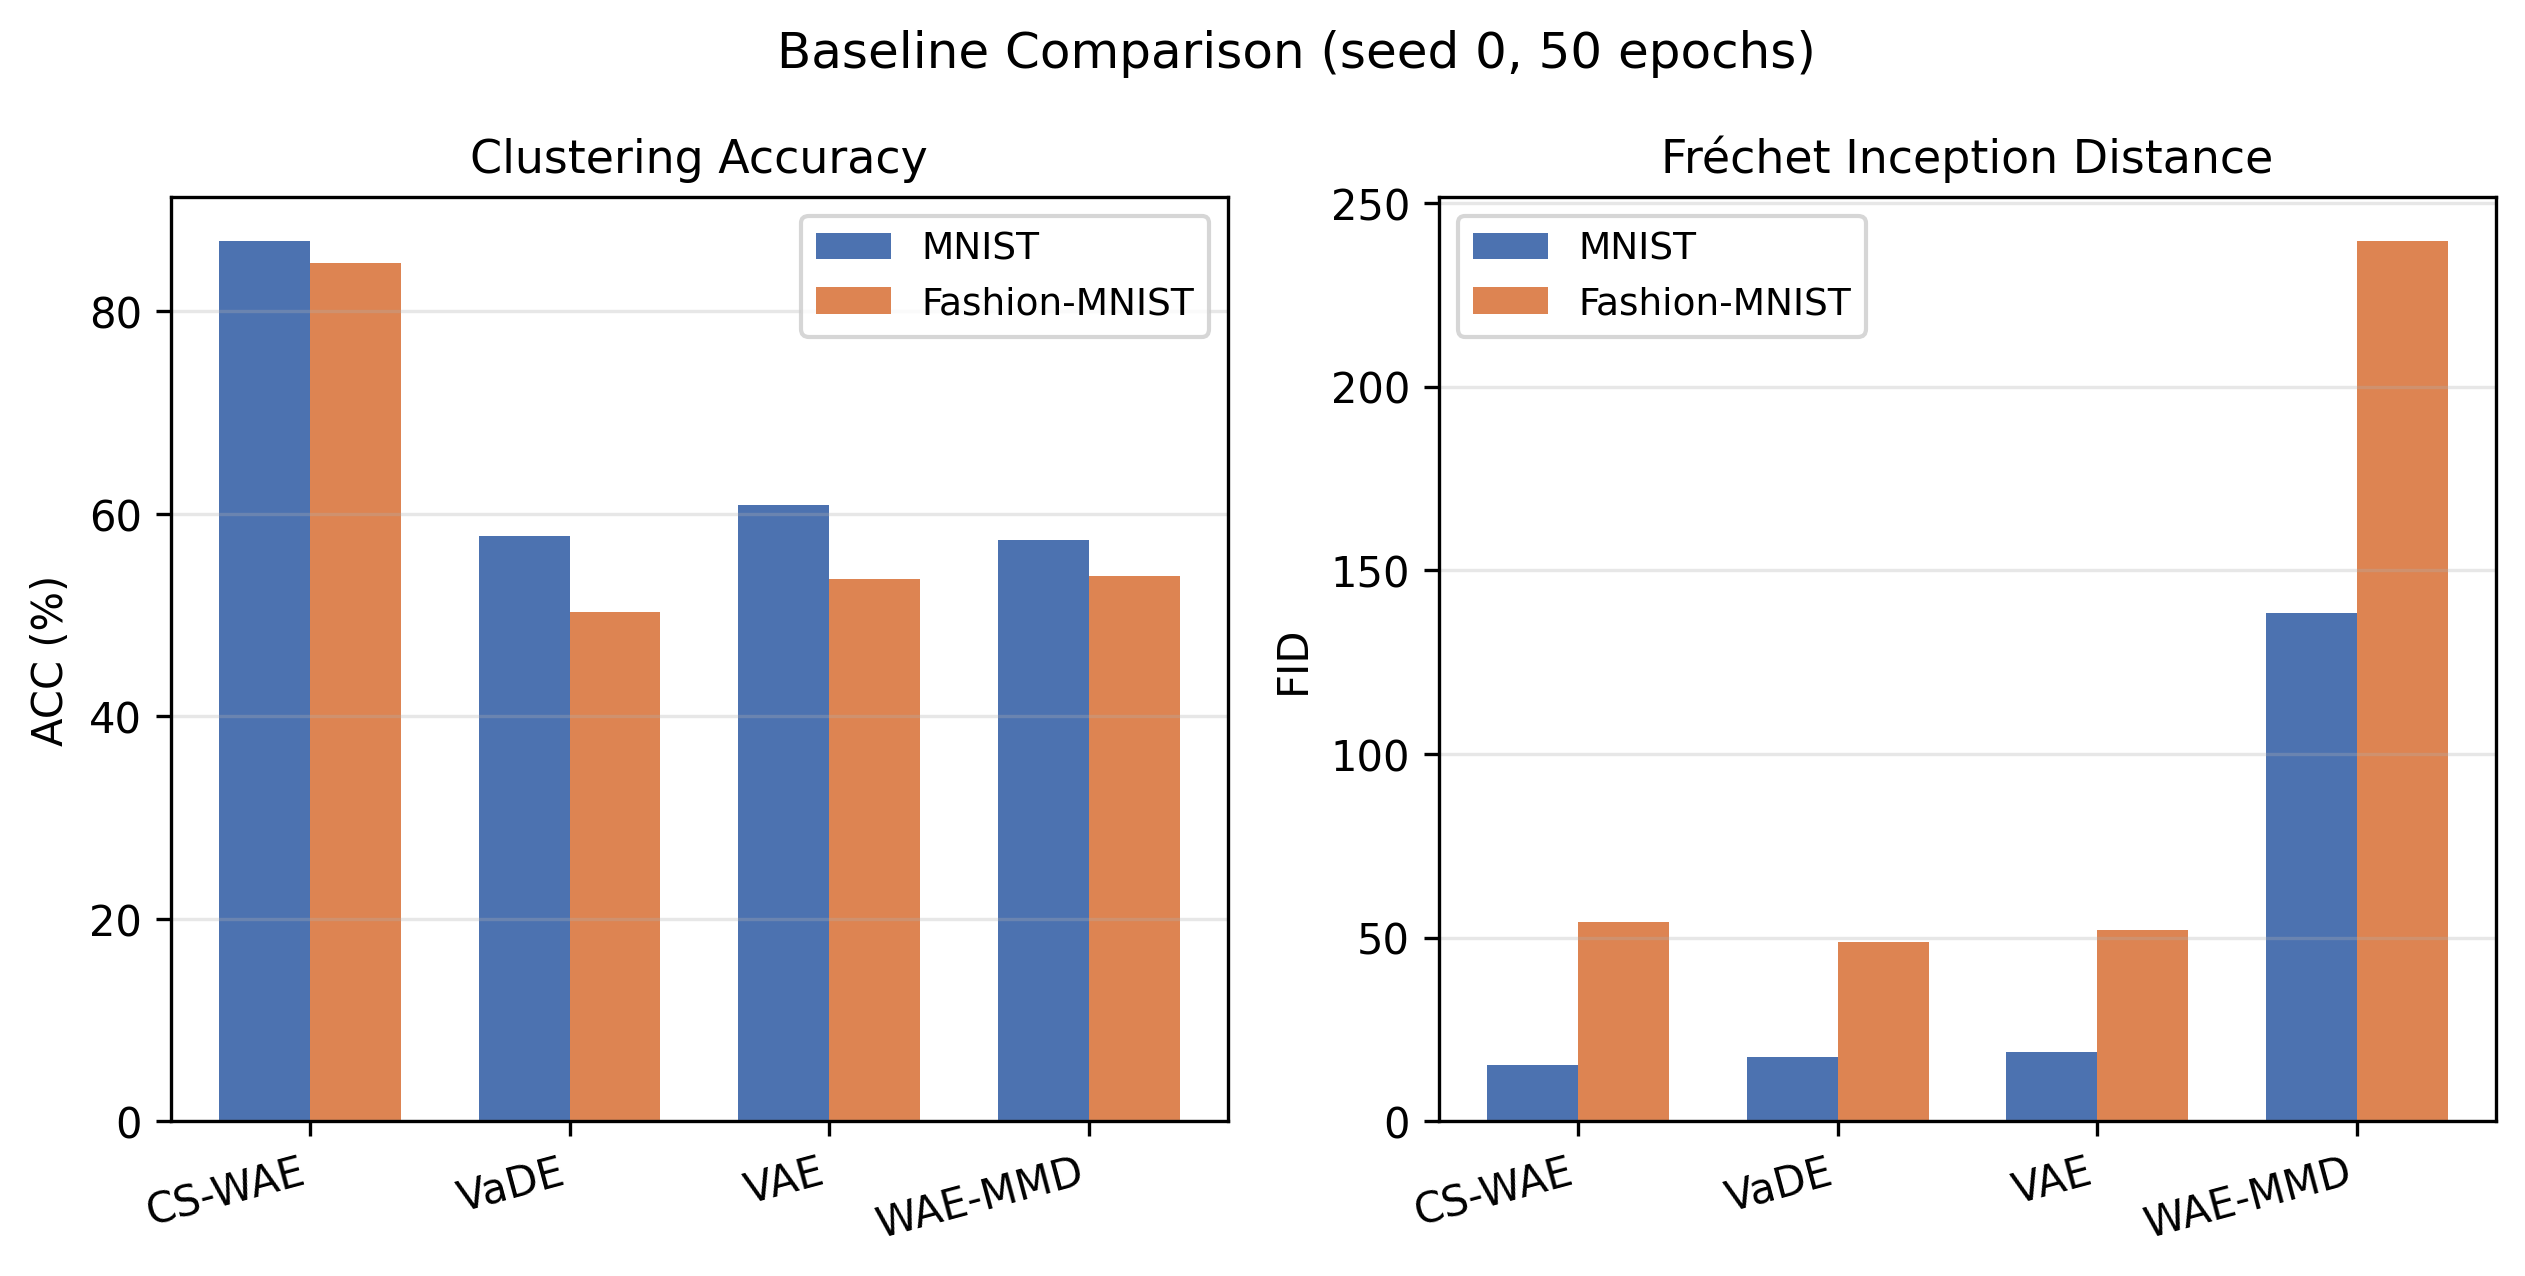
\includegraphics[width=\linewidth]{fig02_baseline_comparison.png}
\caption{Seed-0 baseline comparison. CS-WAE dominates clustering accuracy on both datasets. Its FID is best on MNIST and competitive on Fashion-MNIST, where VaDE obtains the lowest FID but substantially lower clustering accuracy.}
\label{fig:baseline}
\end{figure}

\begin{table}[t]
\centering
\caption{Seed-0 reconstruction SSIM for baseline models. Higher SSIM does not necessarily imply better generated samples or better clustering.}
\label{tab:ssim}
\begin{tabular}{llc}
\toprule
Dataset & Method & SSIM$\uparrow$ \\
\midrule
\multirow{4}{*}{MNIST}
& CS-WAE & 0.891 \\
& VAE & 0.909 \\
& VaDE & 0.909 \\
& WAE-MMD & \textbf{0.942} \\
\midrule
\multirow{4}{*}{Fashion-MNIST}
& CS-WAE & 0.728 \\
& VAE & 0.773 \\
& VaDE & 0.776 \\
& WAE-MMD & \textbf{0.821} \\
\bottomrule
\end{tabular}
\end{table}

Table~\ref{tab:ssim} exposes a useful negative result. WAE-MMD obtains the best SSIM on both datasets, but it has the worst FID by a large margin and does not produce competitive clustering. This is a concrete example of why reconstruction metrics alone are insufficient for evaluating generative representation learning. A model can learn an encoder-decoder map that preserves pixels, yet fail to make the prior useful. The goal of CS-WAE is not to maximize reconstruction in isolation; it is to make the representation, the decoder, and the sampling distribution agree.

\begin{figure}[t]
\centering
\begin{subfigure}{0.49\linewidth}
    \centering
    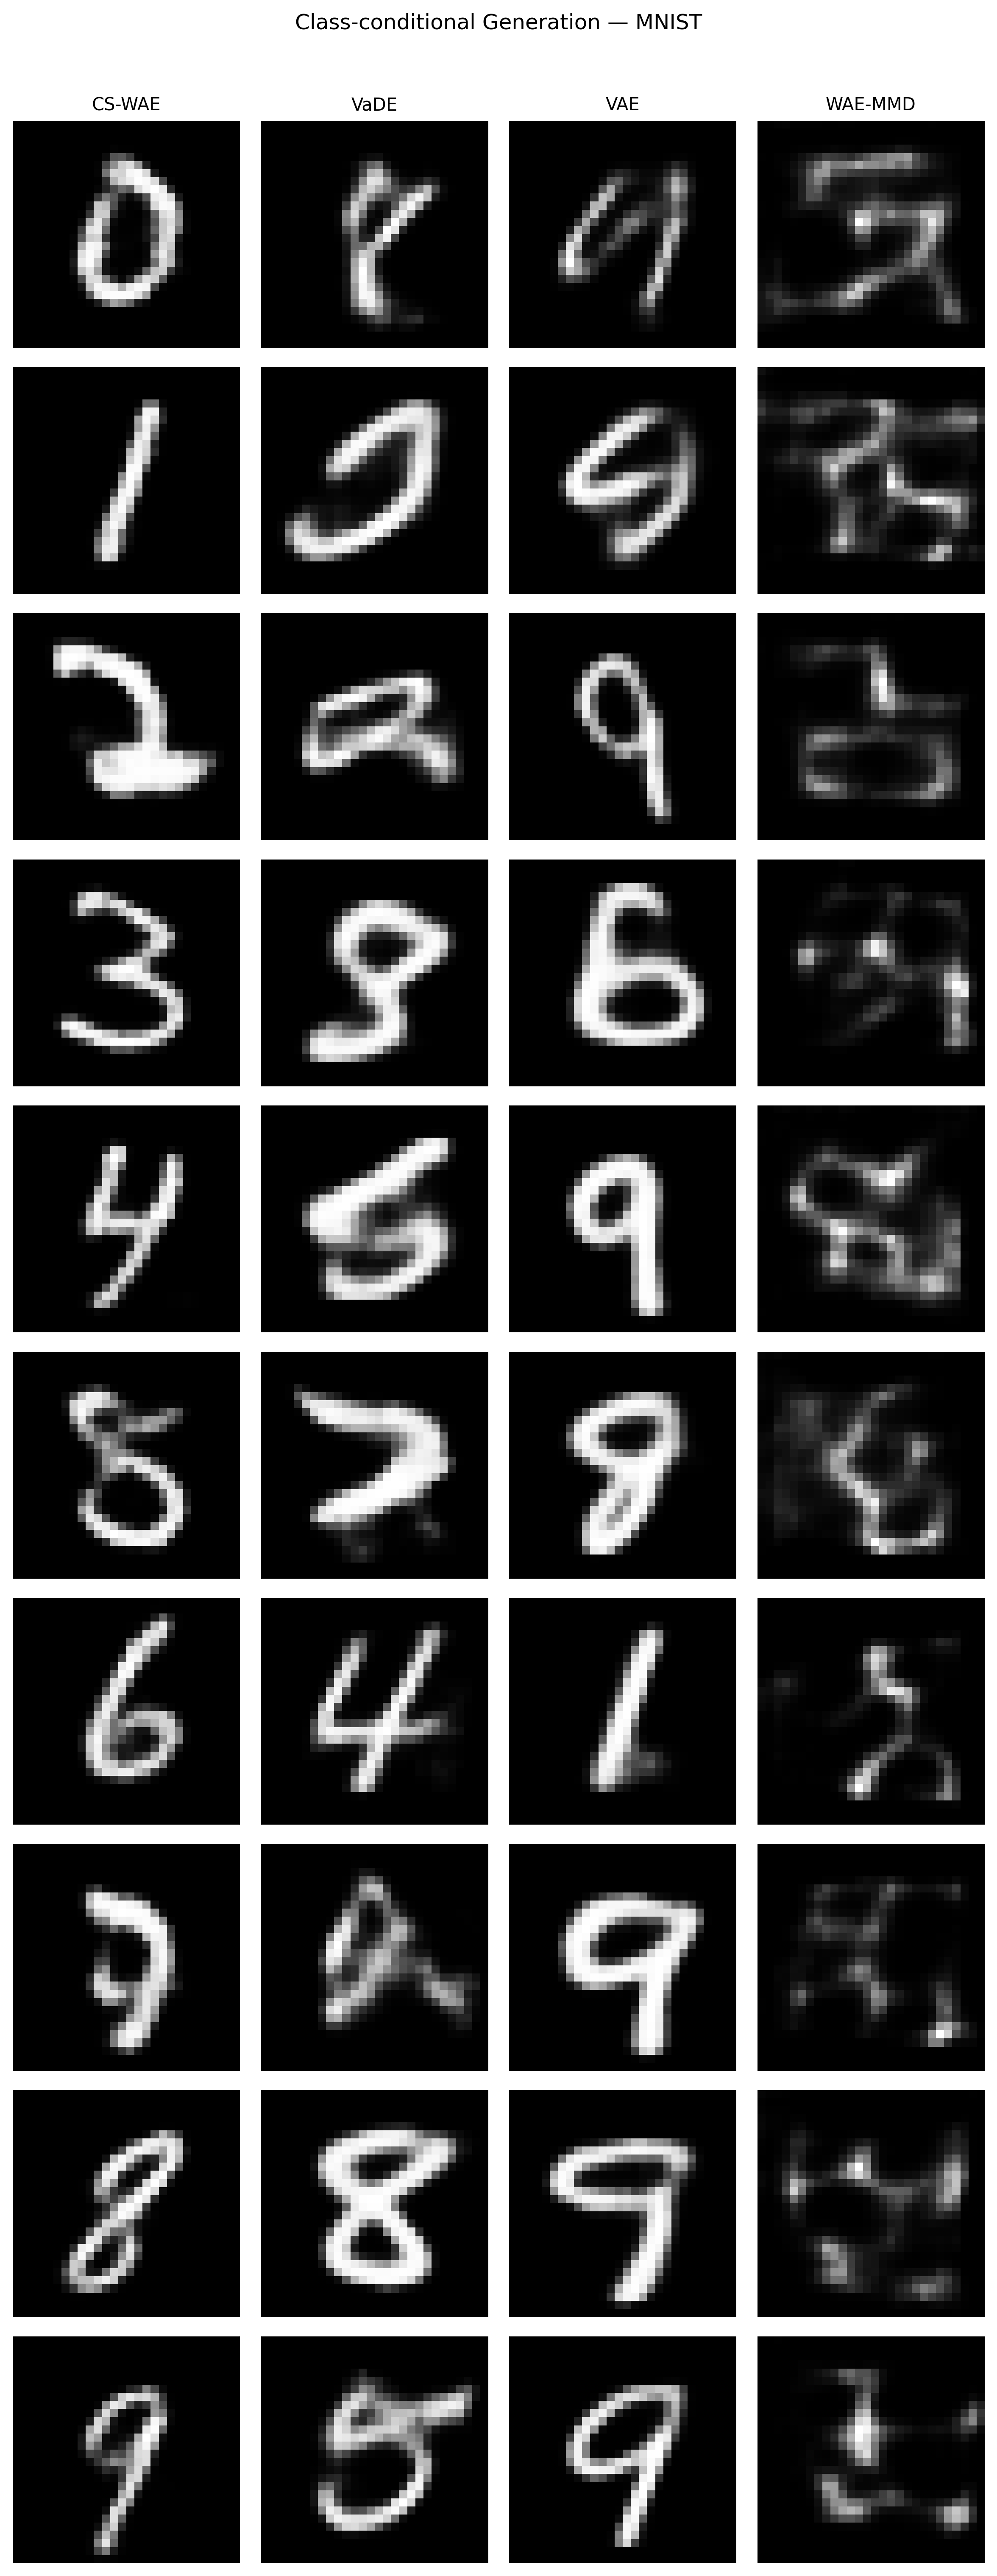
\includegraphics[width=\linewidth]{fig06_generation_grid_mnist.png}
    \caption{MNIST}
\end{subfigure}
\hfill
\begin{subfigure}{0.49\linewidth}
    \centering
    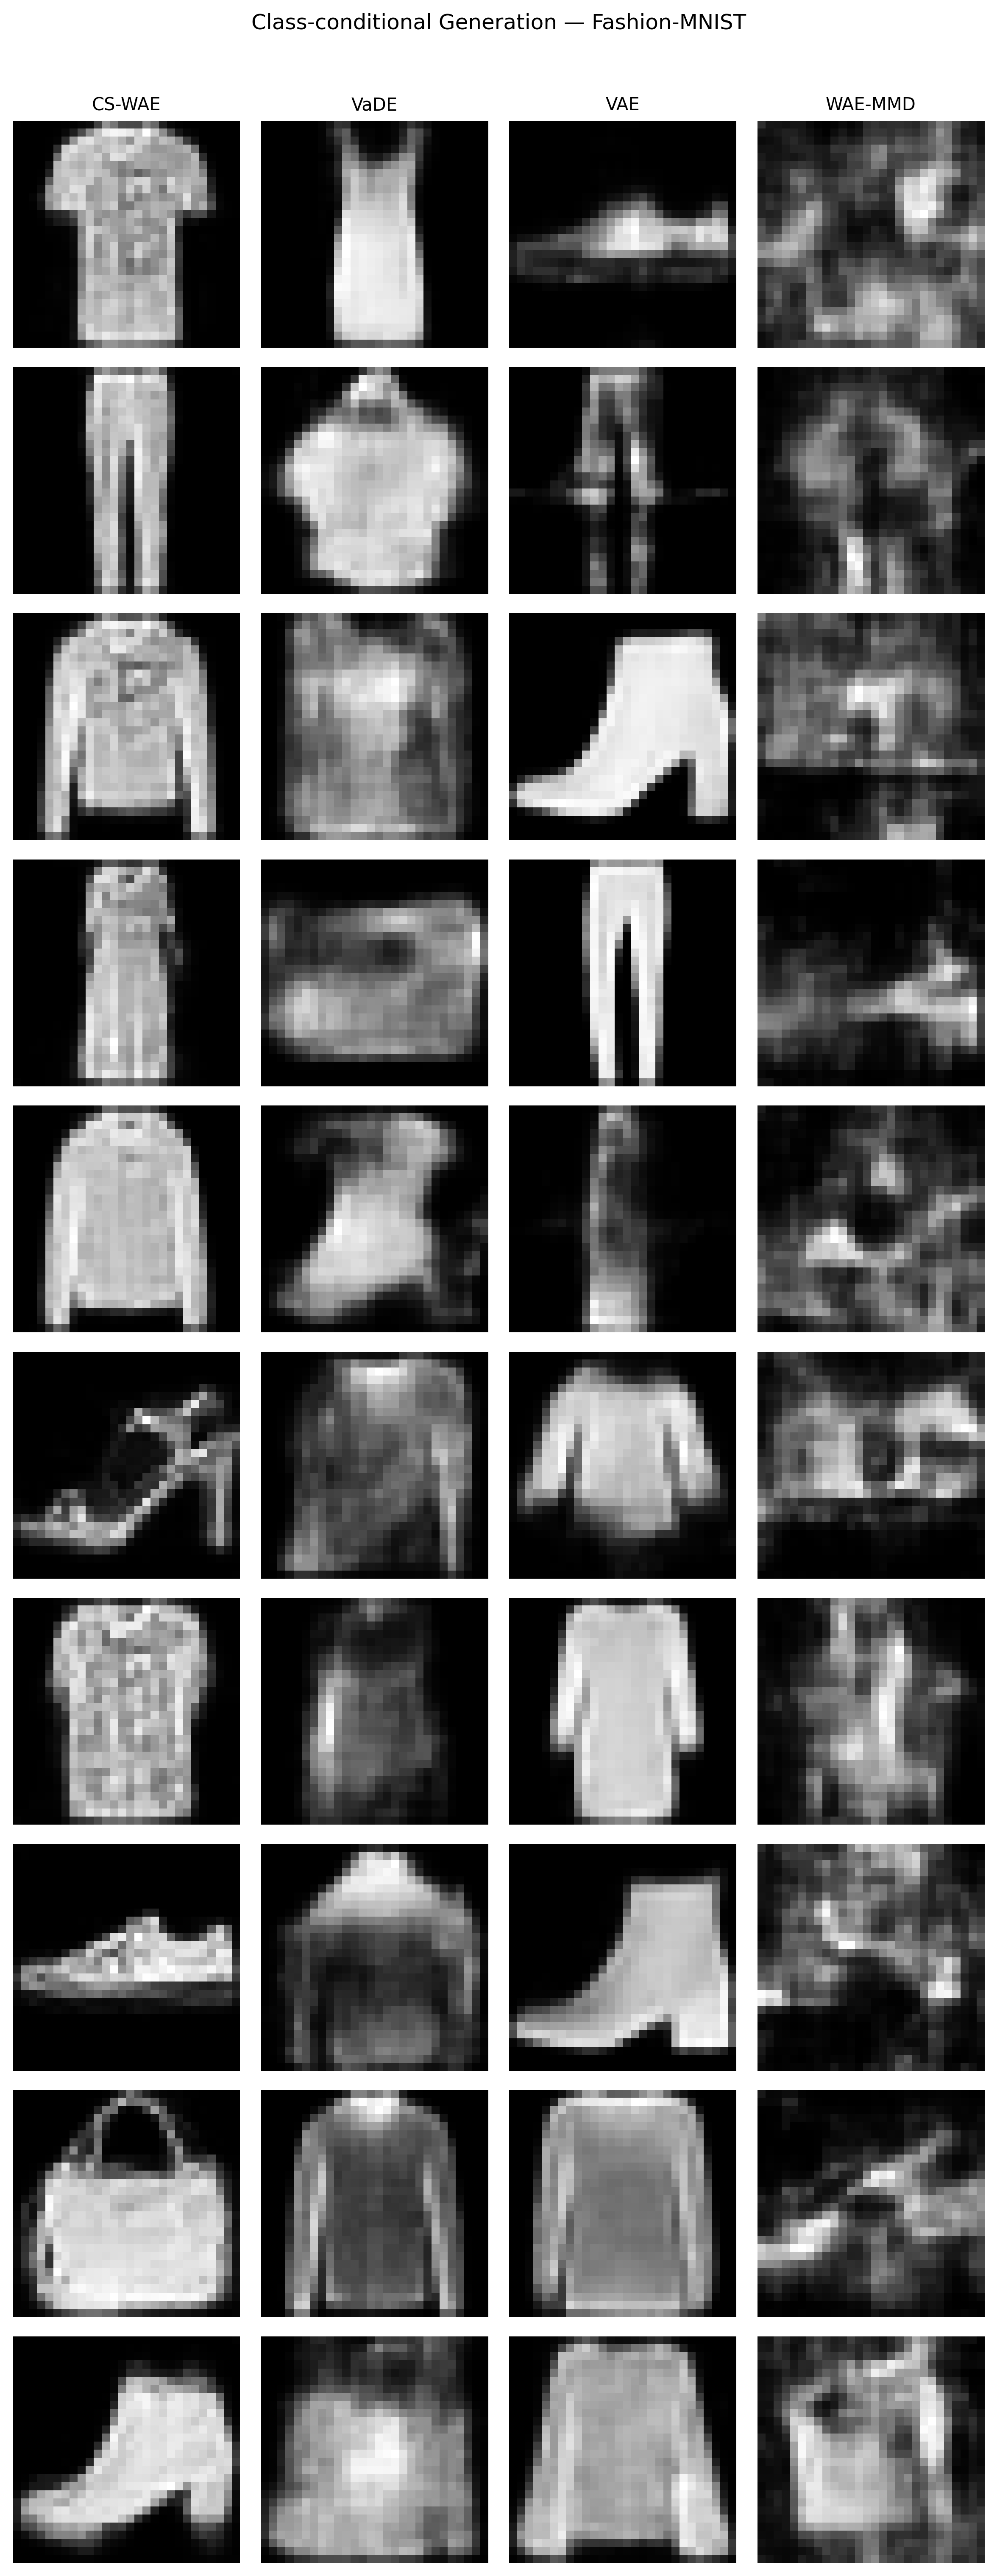
\includegraphics[width=\linewidth]{fig06_generation_grid_fashion_mnist.png}
    \caption{Fashion-MNIST}
\end{subfigure}
\caption{Class-conditional and prior samples. CS-WAE samples are drawn from class-specific Spherical Cauchy priors; VAE and WAE-MMD samples are drawn from a standard Gaussian prior; VaDE samples are drawn from its learned mixture prior.}
\label{fig:generation}
\end{figure}

\subsection{Ablation Study}

\begin{table}[t]
\centering
\caption{Ablation study at seed 0 and 50 epochs. MNIST ablation uses an older, pre-alignment training path and should be interpreted relatively. Fashion-MNIST uses the aligned code path.}
\label{tab:ablation}
\resizebox{\linewidth}{!}{
\begin{tabular}{llccc}
\toprule
Dataset & Variant & ACC$\uparrow$ & NMI$\uparrow$ & FID$\downarrow$ \\
\midrule
\multirow{5}{*}{MNIST}
& Full CS-WAE & 84.1 & 88.7 & 24.6 \\
& w/o supervised MMD & 34.1 & 29.2 & 325.9 \\
& Euclidean & 11.3 & 0.0 & 258.9 \\
& vMF prior & 24.5 & 14.7 & 63.0 \\
& Minimal & 11.3 & 0.0 & 240.1 \\
\midrule
\multirow{5}{*}{Fashion-MNIST}
& Full CS-WAE & 82.2 & 77.4 & 50.1 \\
& w/o supervised MMD & 36.1 & 36.1 & 68.5 \\
& Euclidean & 10.0 & 0.0 & 268.5 \\
& vMF prior & 57.5 & 47.2 & 378.7 \\
& Minimal & 10.0 & 0.0 & 377.3 \\
\bottomrule
\end{tabular}}
\end{table}

Table~\ref{tab:ablation} and Figure~\ref{fig:ablation} isolate the role of each component. Removing supervised MMD causes a large drop in ACC: roughly 50 points on MNIST and 46 points on Fashion-MNIST. This confirms that per-class prior alignment is not a cosmetic addition; it is the mechanism that gives the latent space its class structure. Replacing the hypersphere with a Euclidean variant collapses to near-chance accuracy. The minimal model, which removes both the supervised spherical structure and the Spherical Cauchy prior, also collapses.

The vMF prior behaves differently across datasets. On MNIST it preserves reconstruction well in the extended logs but fails to cluster; on Fashion-MNIST it partially preserves clustering but severely degrades FID. This suggests that the Spherical Cauchy prior provides a more robust compromise between class separation and sampleability. Its heavy-tailed behavior may allow class regions to remain separated without concentrating all mass too aggressively around prior centers.

\begin{figure}[t]
\centering
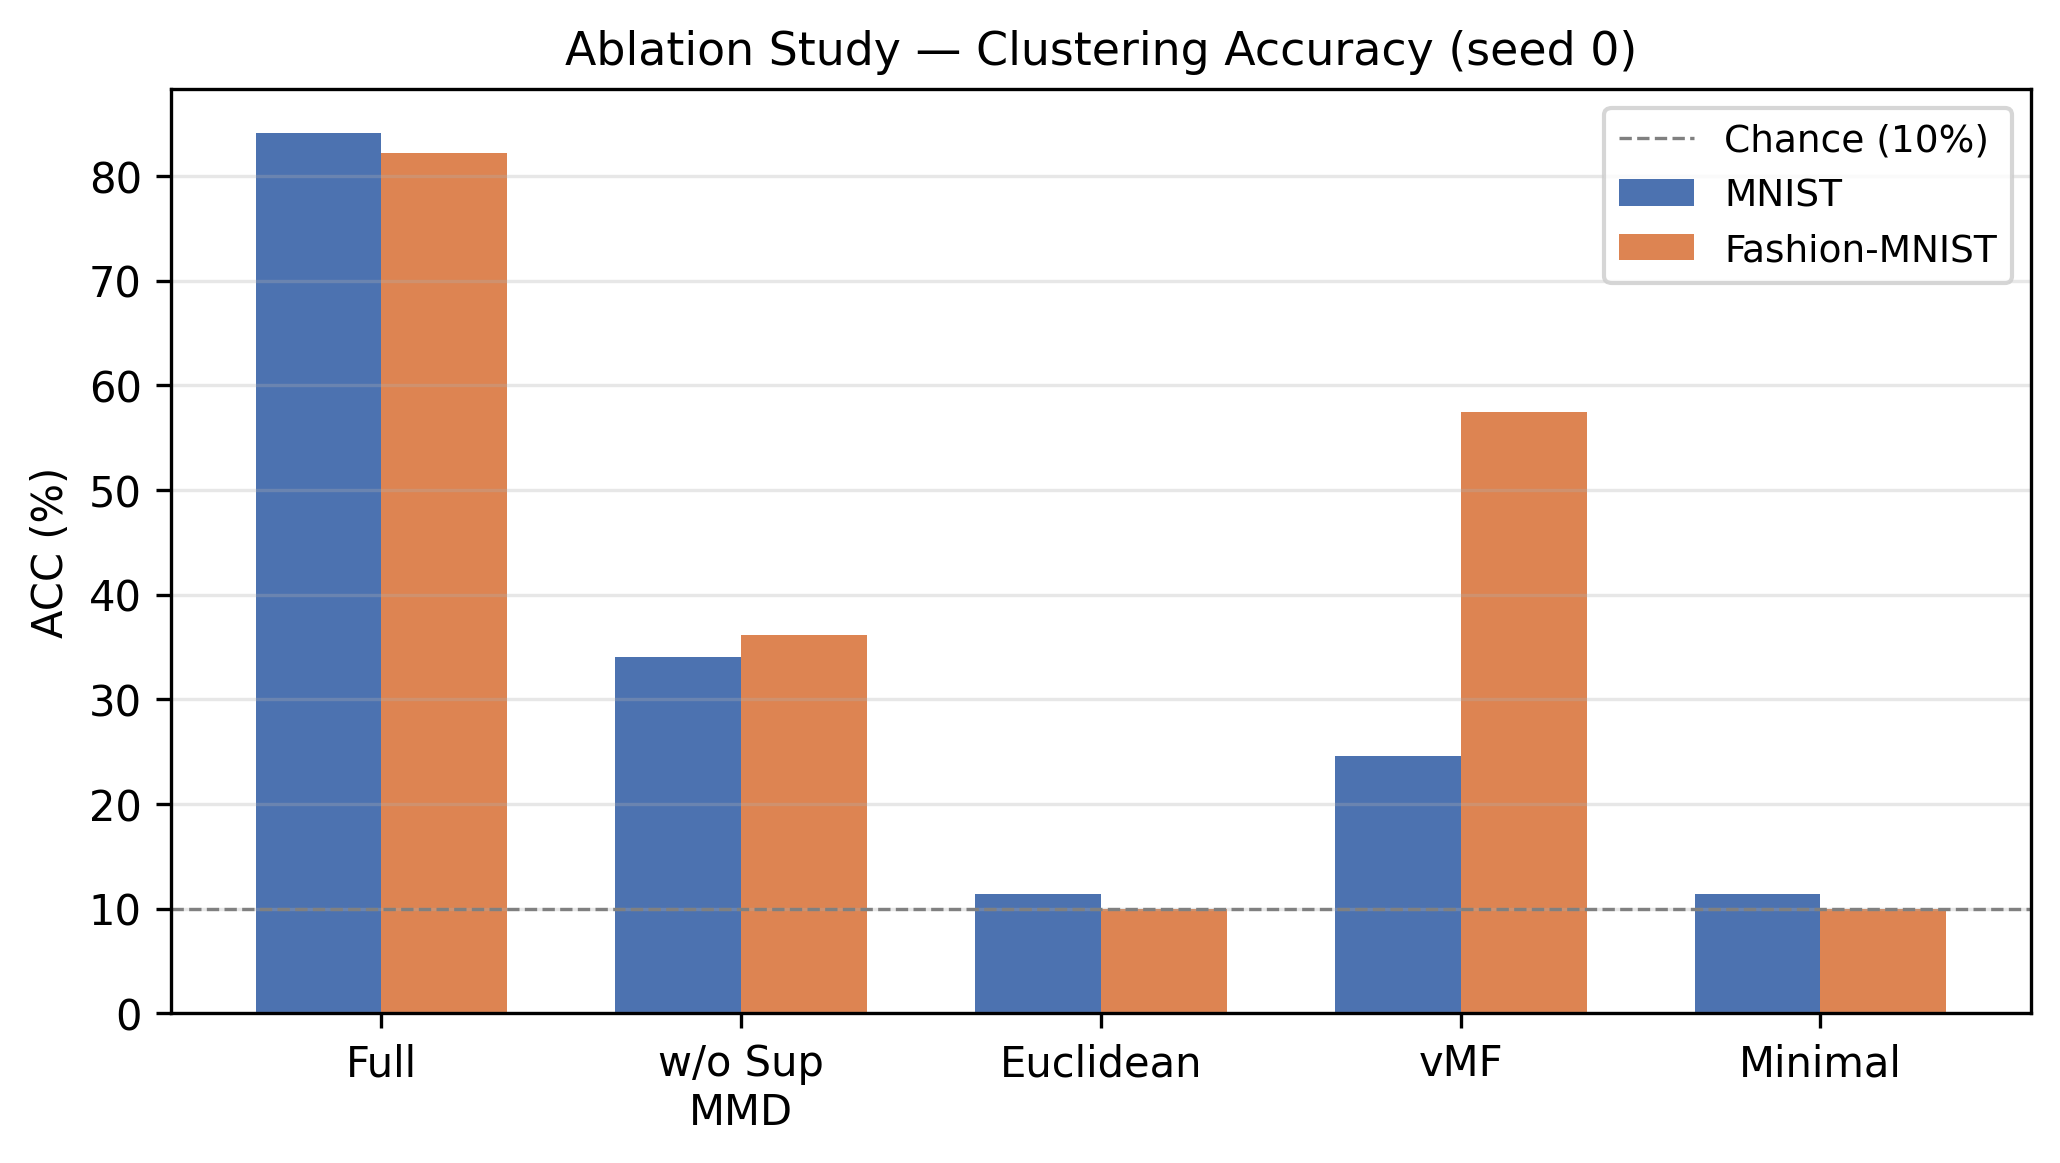
\includegraphics[width=0.92\linewidth]{fig03_ablation_acc.png}
\caption{Ablation accuracy. Supervised MMD and spherical geometry are both essential. Euclidean and minimal variants collapse to chance-level clustering.}
\label{fig:ablation}
\end{figure}

\begin{figure}[t]
\centering
\begin{subfigure}{0.49\linewidth}
    \centering
    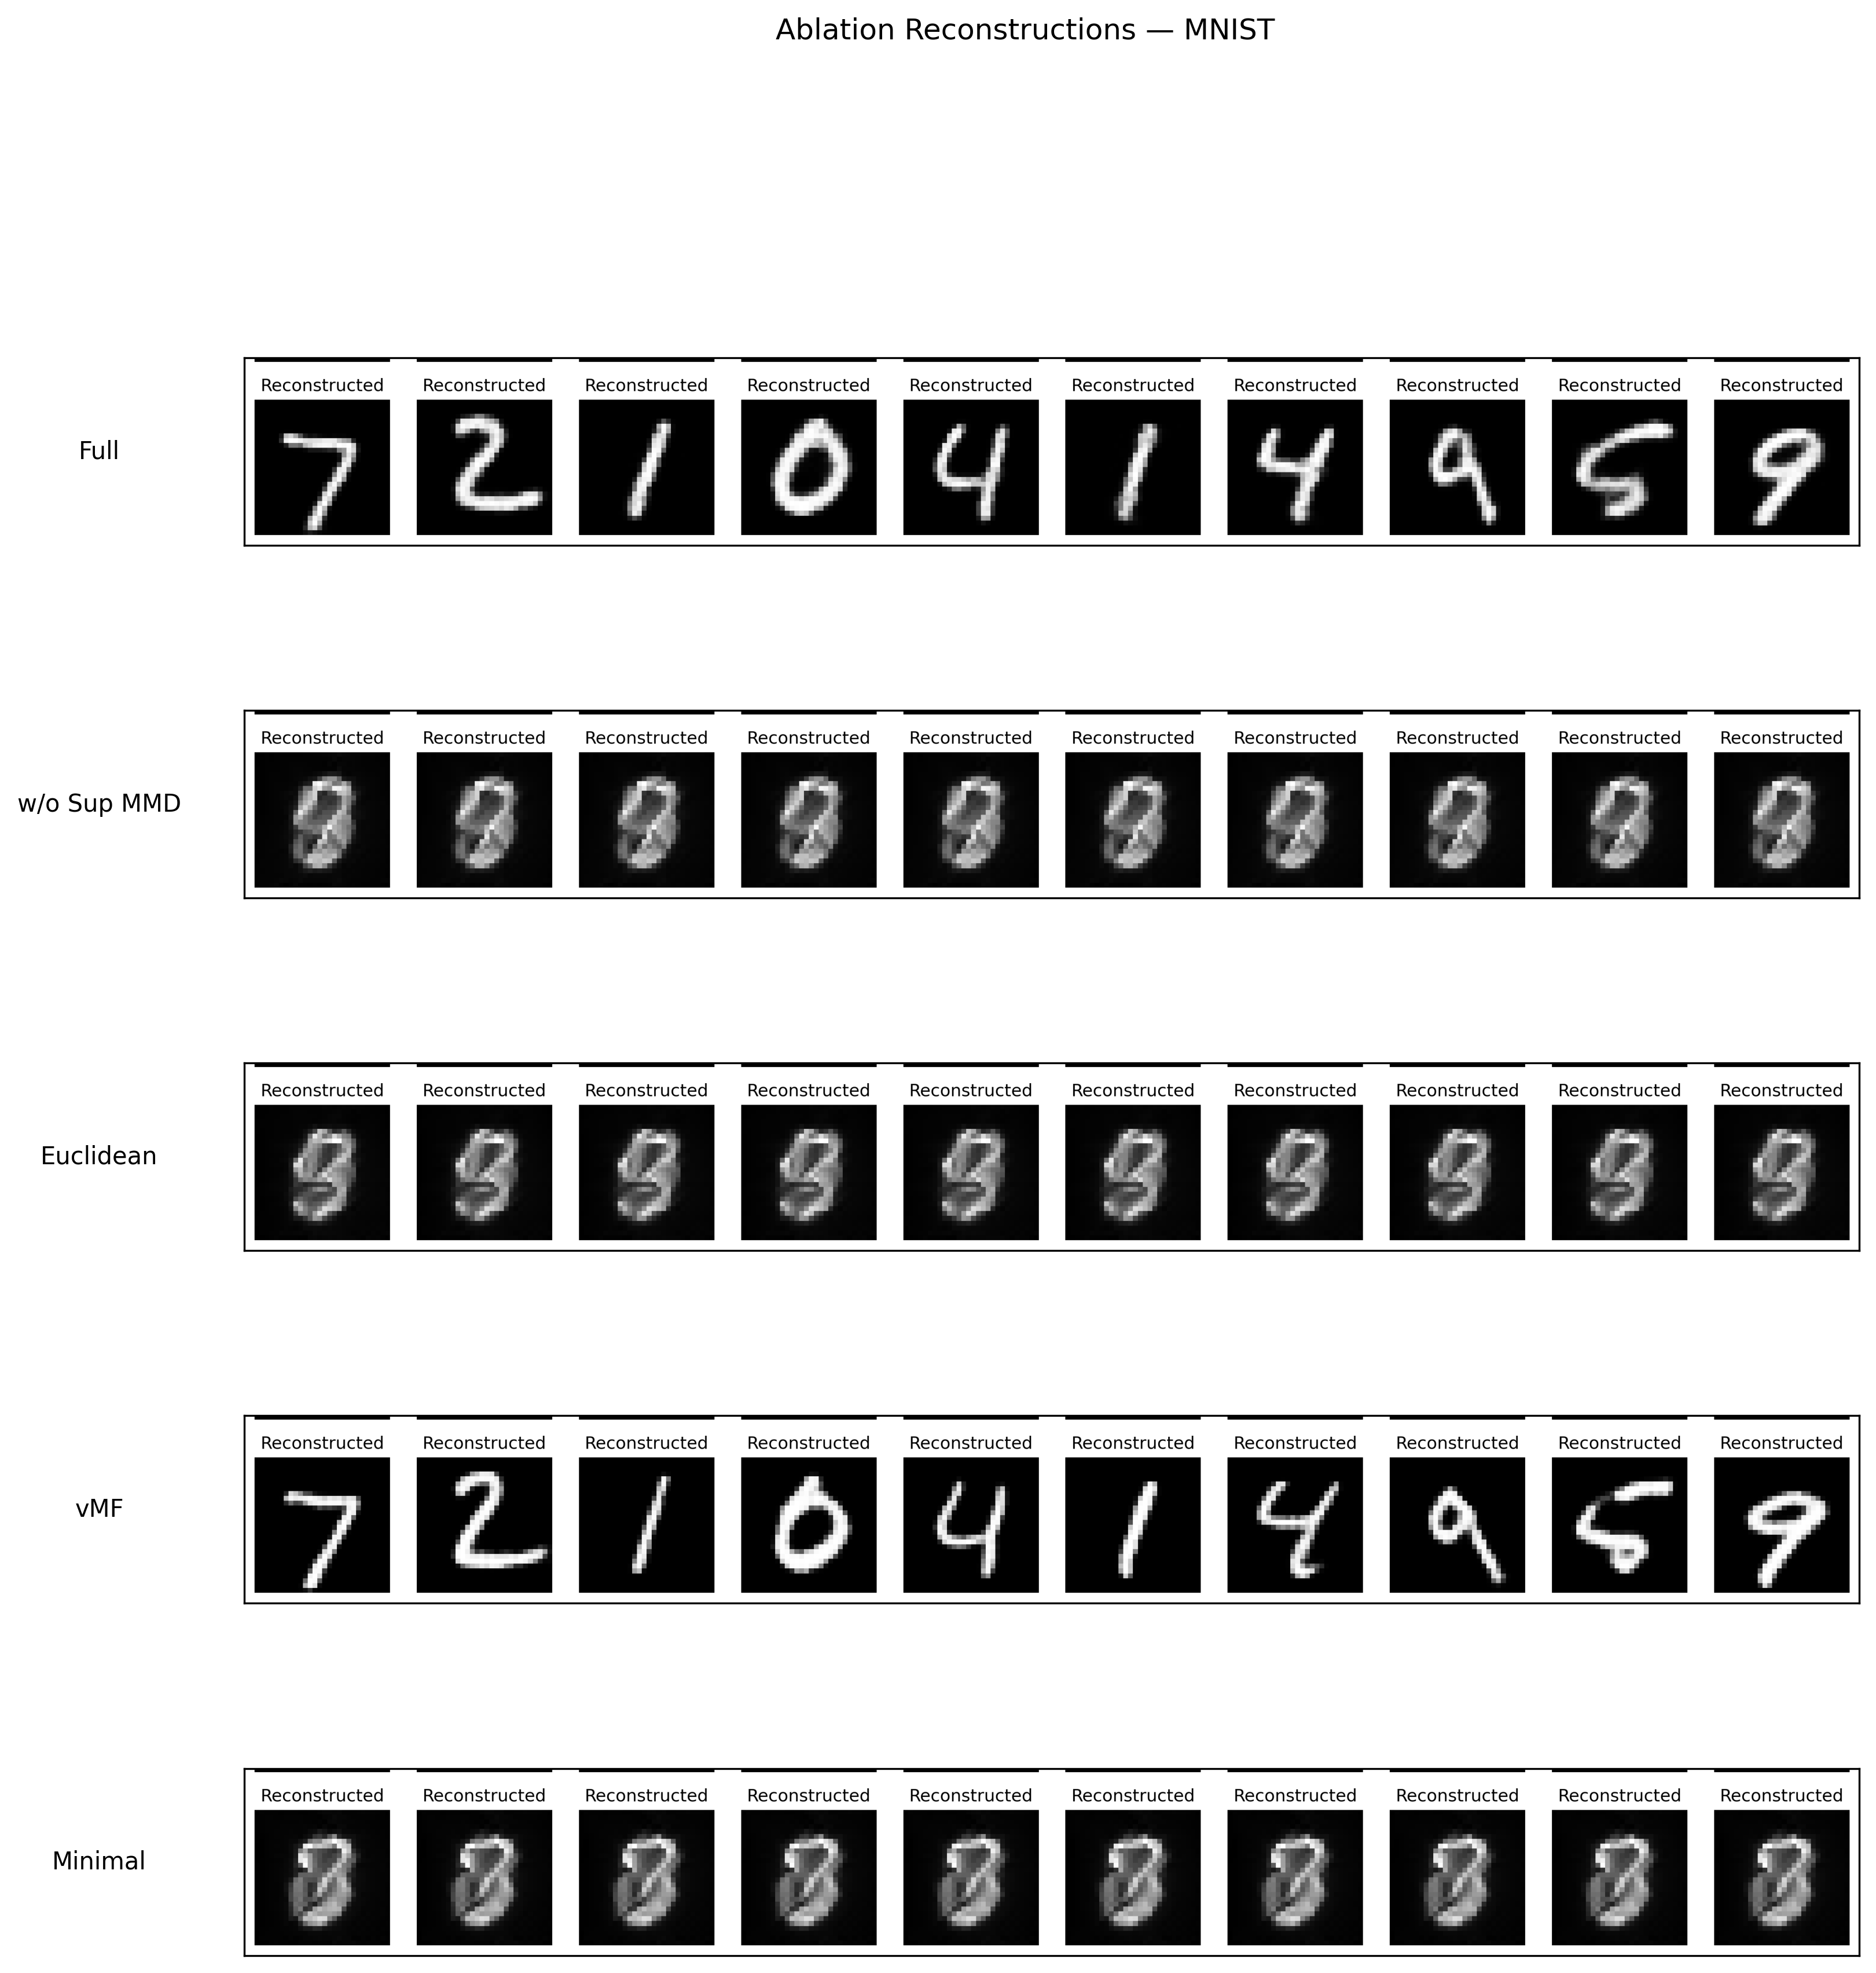
\includegraphics[width=\linewidth]{fig11_ablation_recon_mnist.png}
    \caption{MNIST}
\end{subfigure}
\hfill
\begin{subfigure}{0.49\linewidth}
    \centering
    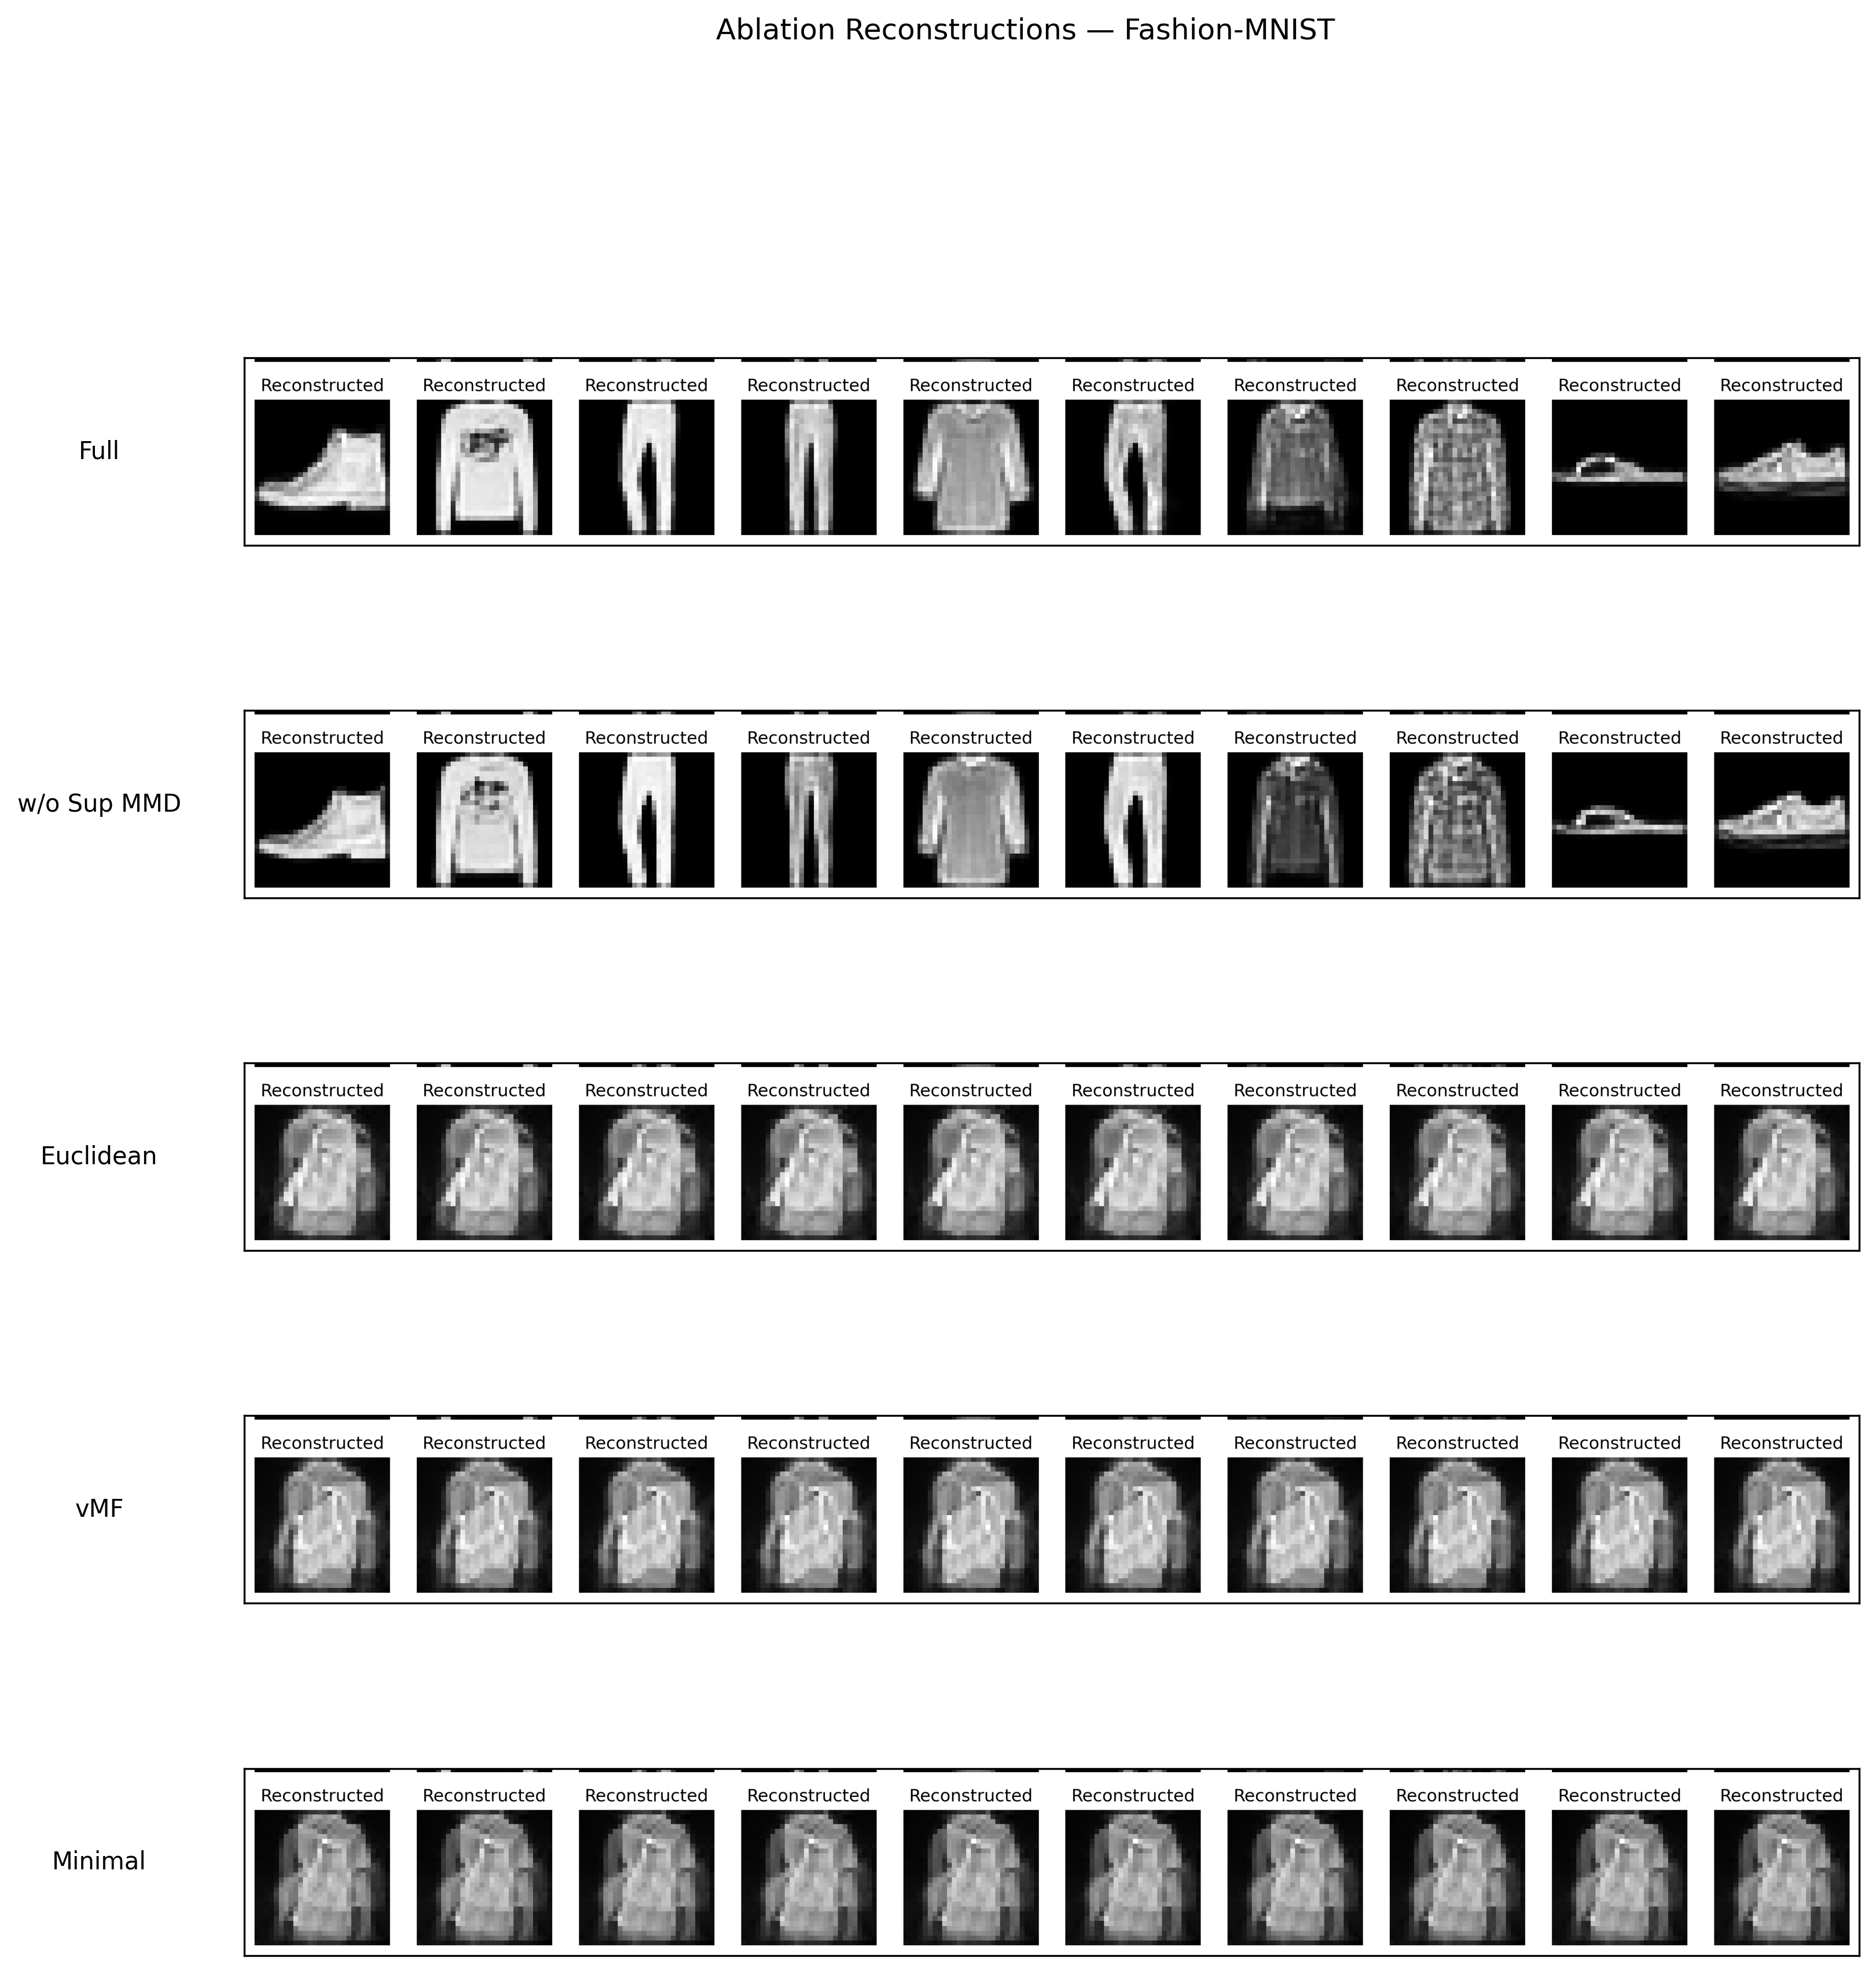
\includegraphics[width=\linewidth]{fig11_ablation_recon_fashion_mnist.png}
    \caption{Fashion-MNIST}
\end{subfigure}
\caption{Ablation reconstructions. Collapsed variants often reconstruct poorly or produce visually unstable outputs, supporting the quantitative collapse observed in Table~\ref{tab:ablation}.}
\label{fig:ablation-recon}
\end{figure}

\subsection{Cross-Dataset Behavior}

The comparison between MNIST and Fashion-MNIST is informative because the two datasets share the same image size, number of classes, and train-test split size, but differ in visual ambiguity. MNIST digits are usually separated by global stroke shape. Fashion-MNIST classes include visually similar objects such as shirts, coats, pullovers, sandals, sneakers, and ankle boots. A method that works only on MNIST may be exploiting a relatively easy geometry.

CS-WAE degrades on Fashion-MNIST, as expected, but the nature of the degradation is revealing. Mean ACC drops from $92.9$ to $79.0$, and ARI drops from $88.5$ to $69.0$, indicating that fine-grained cluster assignment becomes harder. FID increases from $19.4$ to $50.7$, reflecting the higher visual diversity and texture complexity of fashion images. However, the baseline gap in ACC does not shrink; it grows from roughly 26--29 points on MNIST to 31--34 points on Fashion-MNIST. This suggests that the class-structured spherical prior is especially useful when Euclidean latent baselines struggle to separate visually overlapping categories.

The ablations also transfer across datasets. Removing supervised MMD collapses both datasets to the mid-30s in ACC, while Euclidean and minimal variants fall to chance level. The vMF prior is the only component whose behavior is strongly dataset-dependent. This dataset dependence is useful evidence rather than a nuisance: it shows that simply choosing a hyperspherical distribution is insufficient. The particular prior family matters, and the Spherical Cauchy prior is more robust in the current experiments.

\subsection{Latent Space Visualization}

Figure~\ref{fig:tsne} visualizes latent spaces with t-SNE for CS-WAE, VaDE, and VAE. CS-WAE produces compact and mostly separated regions, while VaDE and VAE show more overlap. These visualizations match the quantitative clustering results: the main benefit of CS-WAE is not simply lower reconstruction error, but a latent geometry that exposes class structure to a simple K-means evaluator.

\begin{figure}[t]
\centering
\begin{subfigure}{0.49\linewidth}
    \centering
    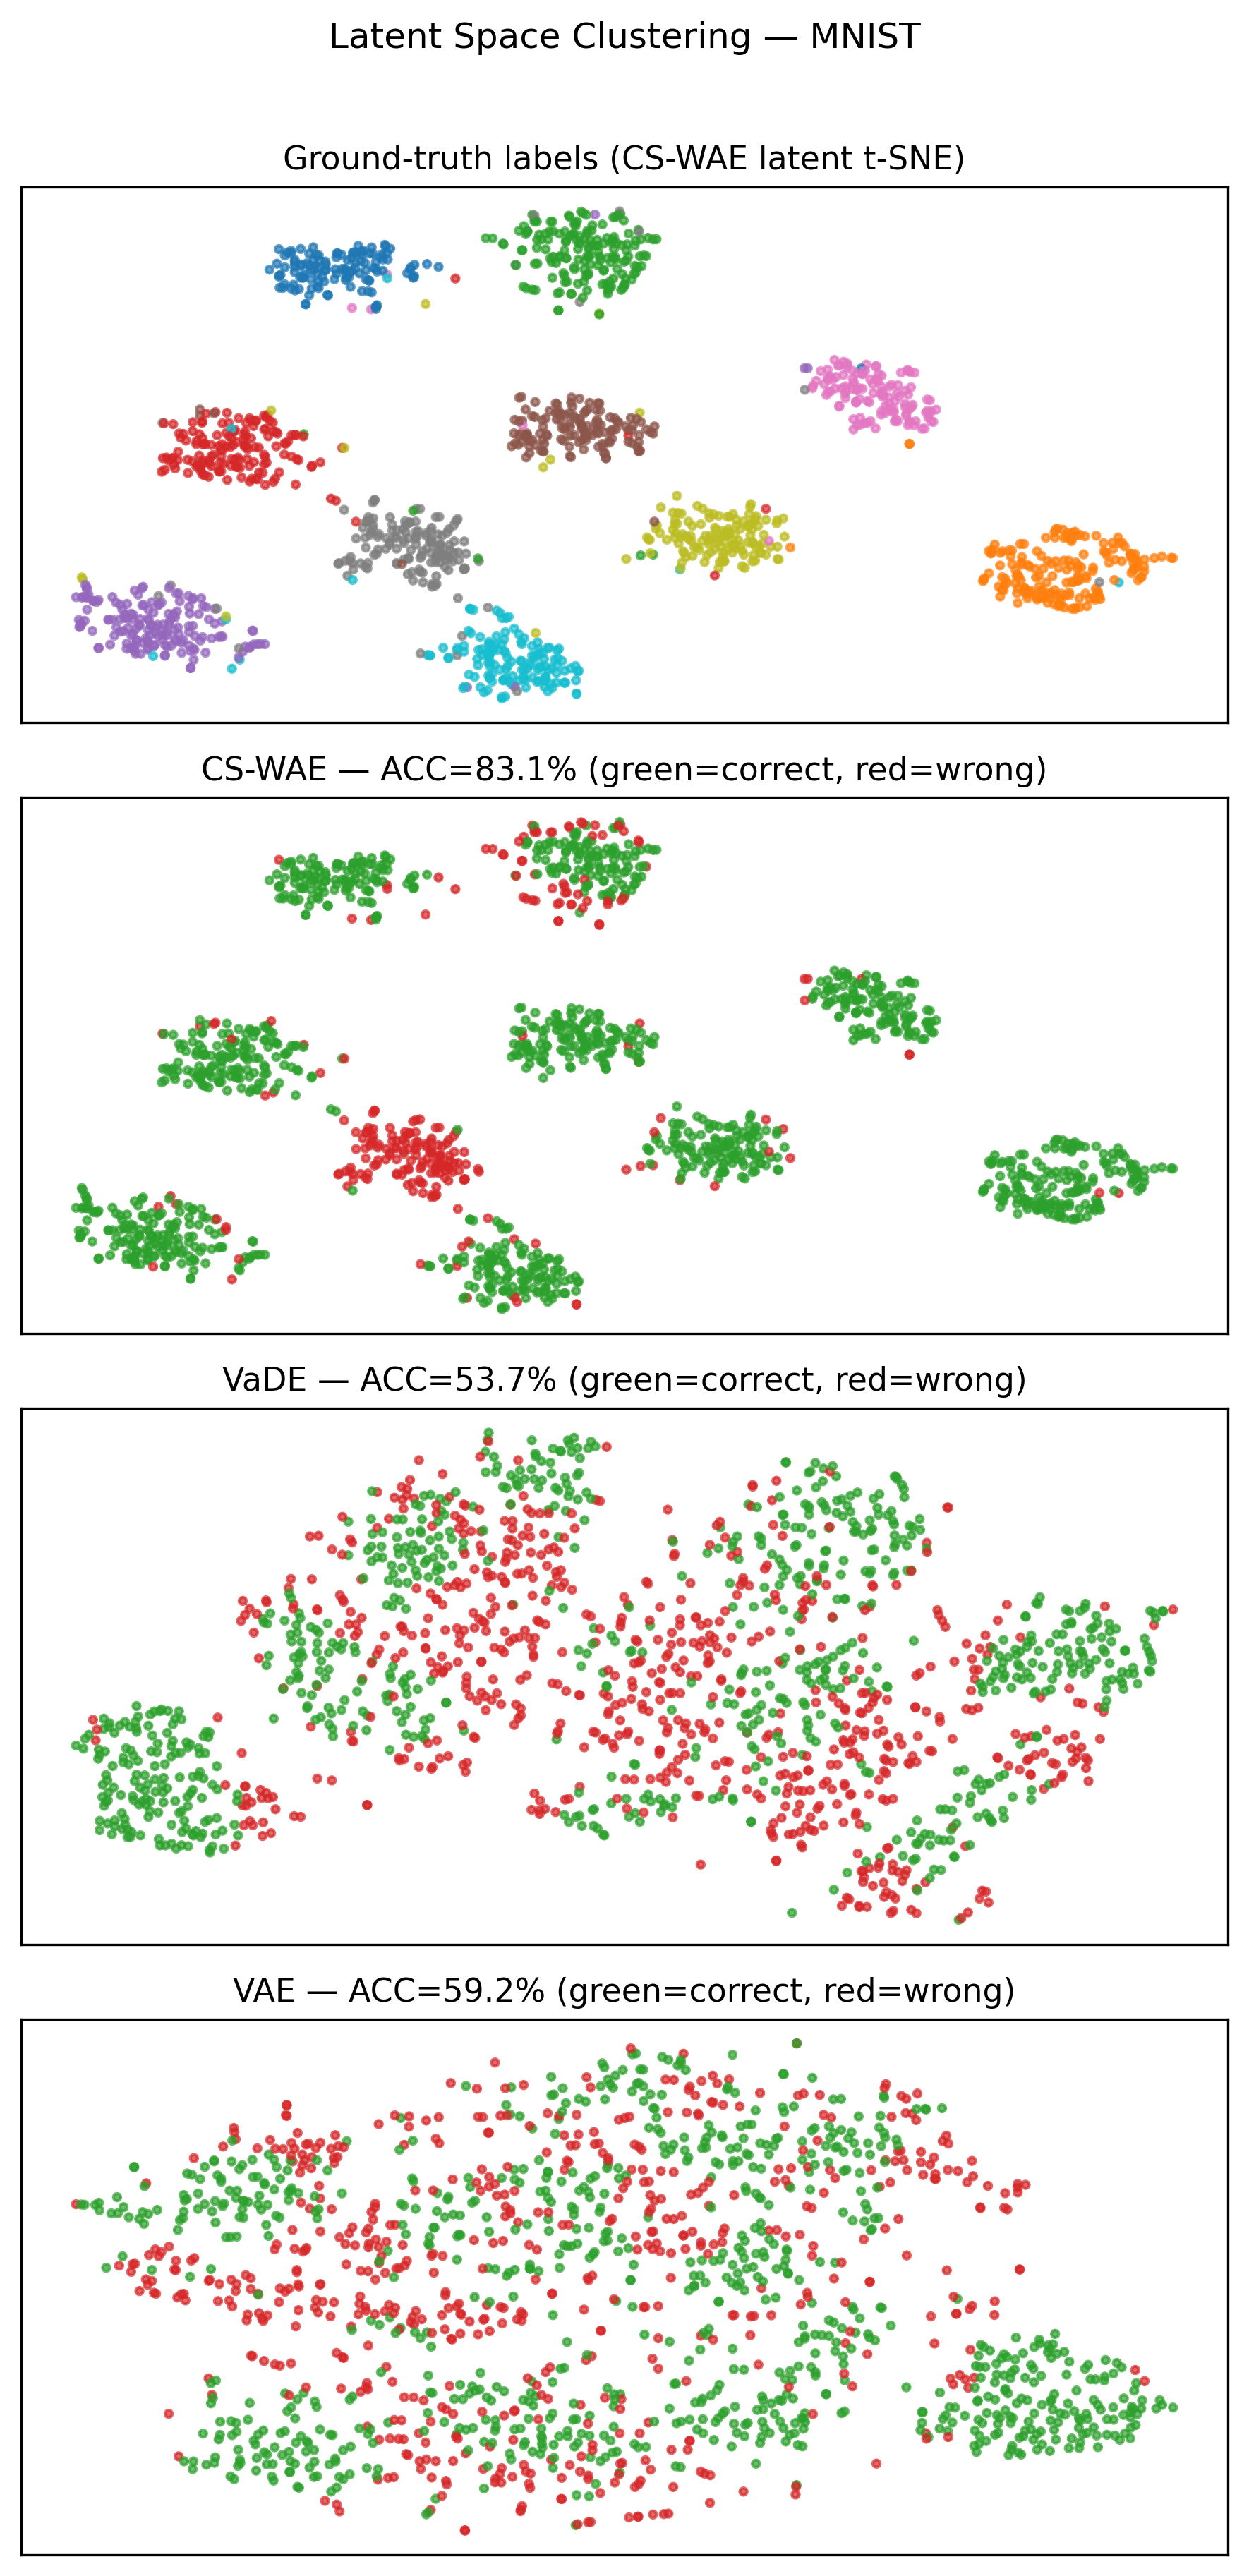
\includegraphics[width=\linewidth]{fig04_tsne_clustering_mnist.png}
    \caption{MNIST}
\end{subfigure}
\hfill
\begin{subfigure}{0.49\linewidth}
    \centering
    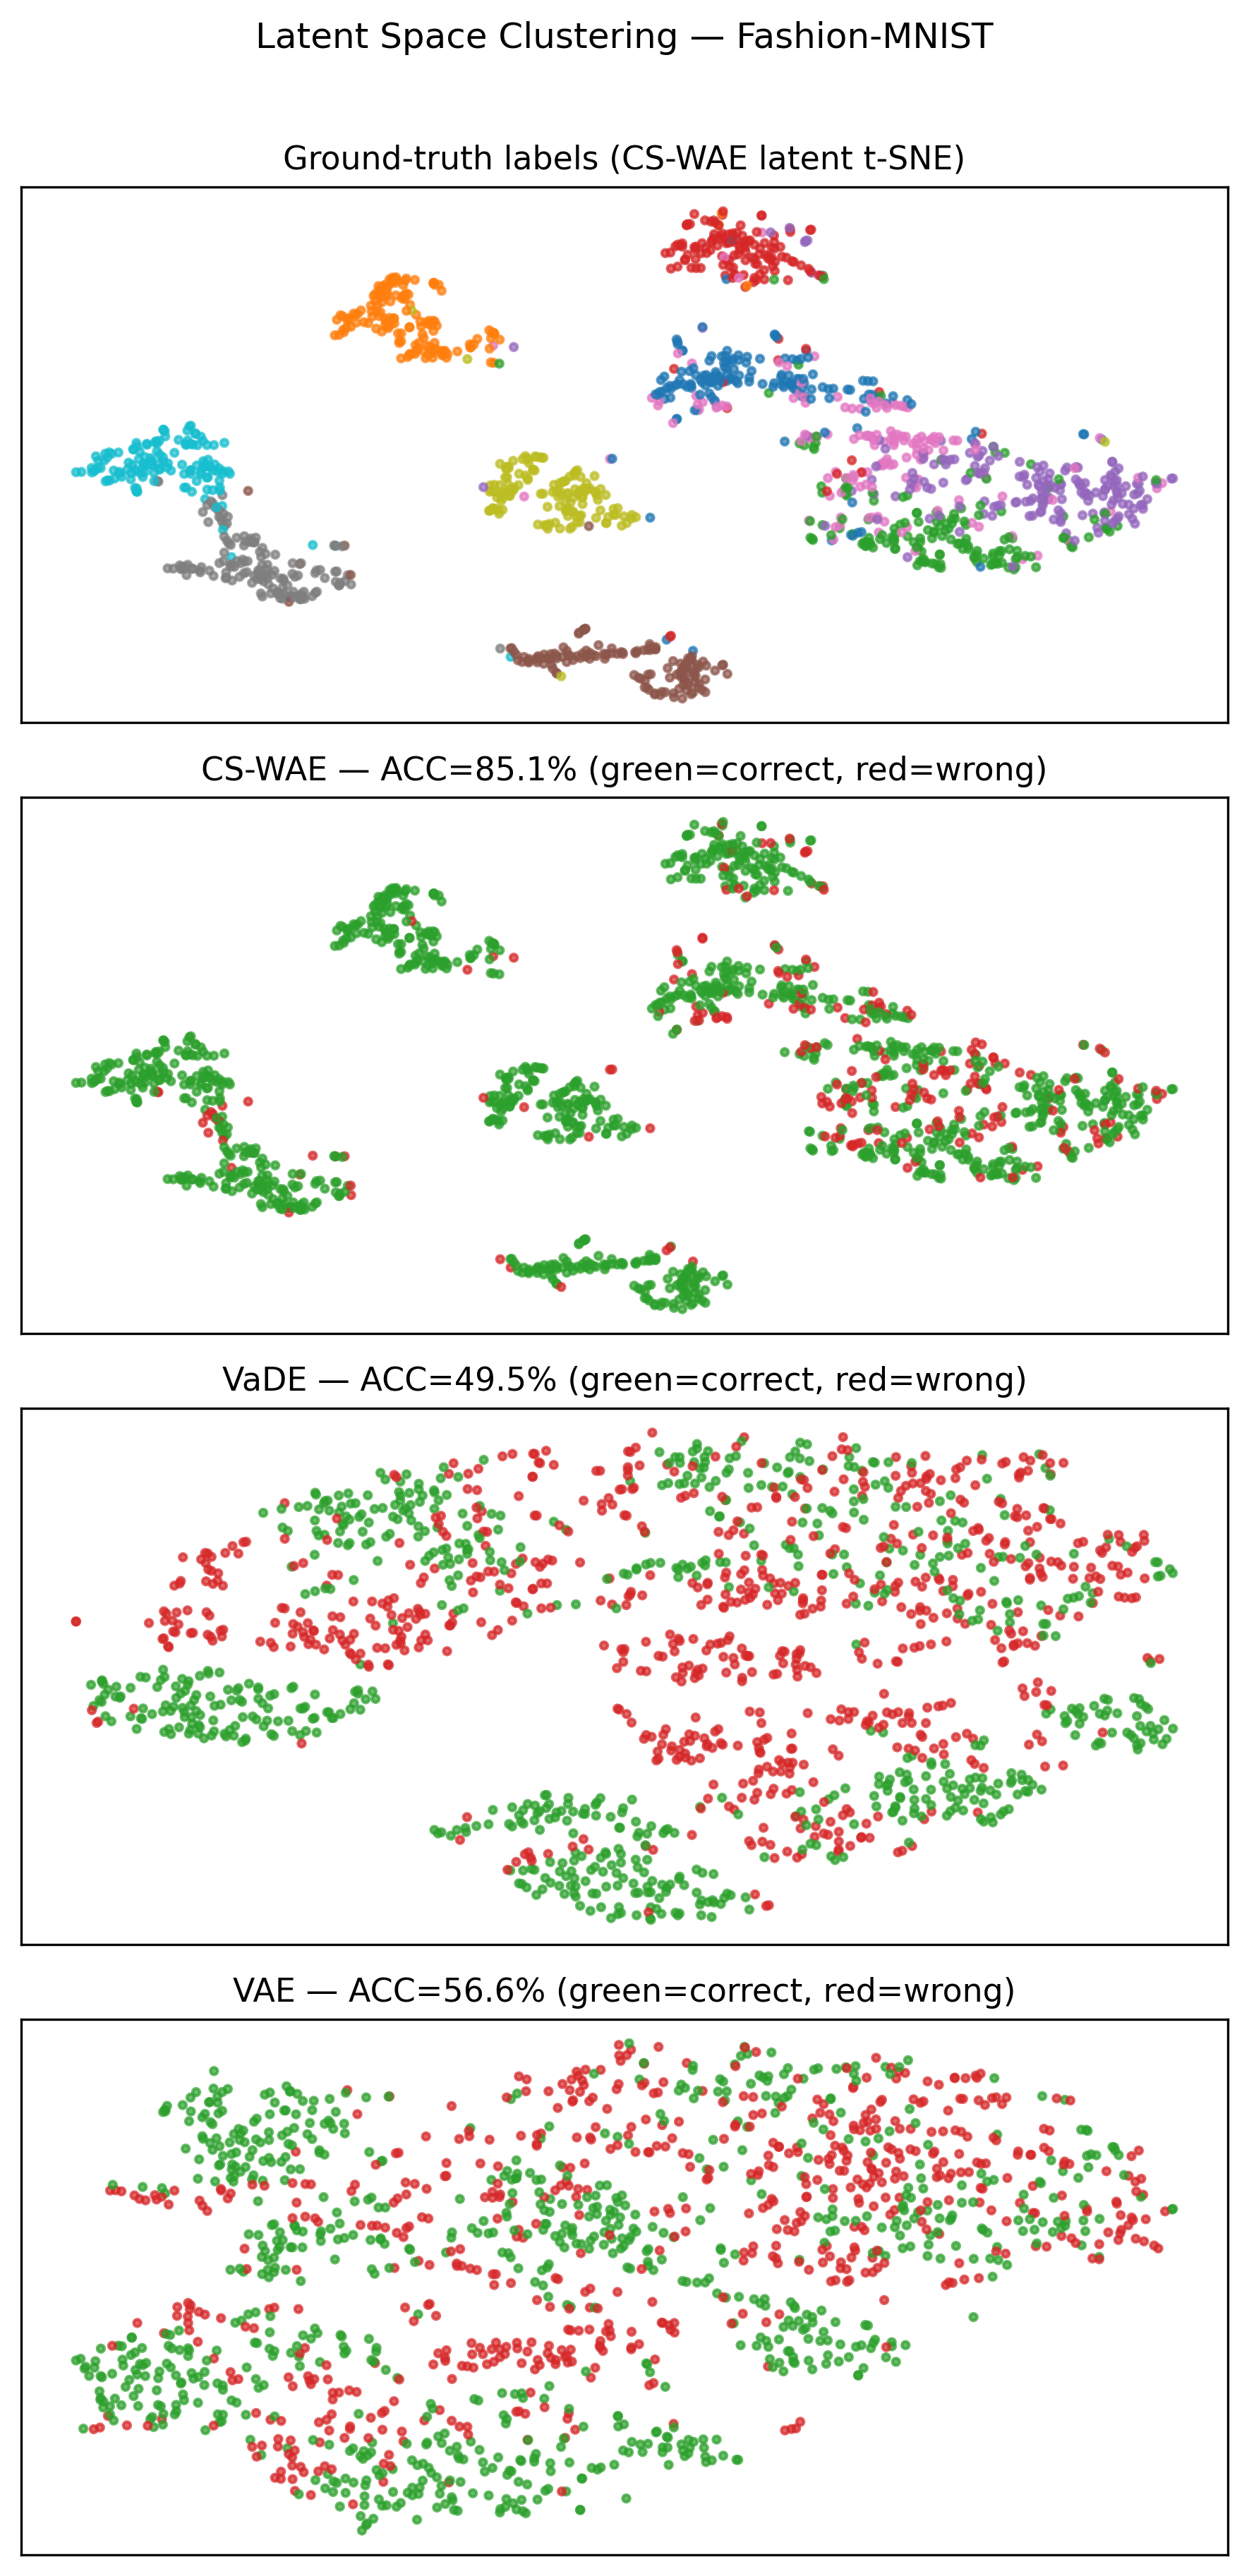
\includegraphics[width=\linewidth]{fig04_tsne_clustering_fashion_mnist.png}
    \caption{Fashion-MNIST}
\end{subfigure}
\caption{Latent t-SNE visualizations for CS-WAE and baselines. The figure uses sampled subsets for readability; therefore the ACC annotations can differ slightly from the full-test metrics in Table~\ref{tab:baselines}.}
\label{fig:tsne}
\end{figure}

\subsection{Sample Quality and Failure Modes}

Figure~\ref{fig:fid-samples} shows random generated samples used for FID inspection. The qualitative pattern is consistent with the metrics. WAE-MMD can reconstruct well but often produces weak prior samples, especially on Fashion-MNIST. VaDE produces competitive samples on Fashion-MNIST but its latent space is less aligned with the K-means clustering protocol. CS-WAE samples are not perfect, particularly for visually ambiguous fashion classes, but they remain tied to a class-structured prior that also supports clustering.

This distinction is central to the model's purpose. If the objective were only unconditional sample quality, a pure generative model or a stronger decoder might be preferable. If the objective were only supervised classification, a discriminative CNN would be much simpler and stronger. CS-WAE targets the middle ground: a generative latent space that exposes class structure while remaining samplable. The failure cases therefore tend to appear when these requirements conflict, such as fashion categories with high intra-class variation or pairs of classes whose visual differences are local rather than global.

\begin{figure}[t]
\centering
\begin{subfigure}{0.49\linewidth}
    \centering
    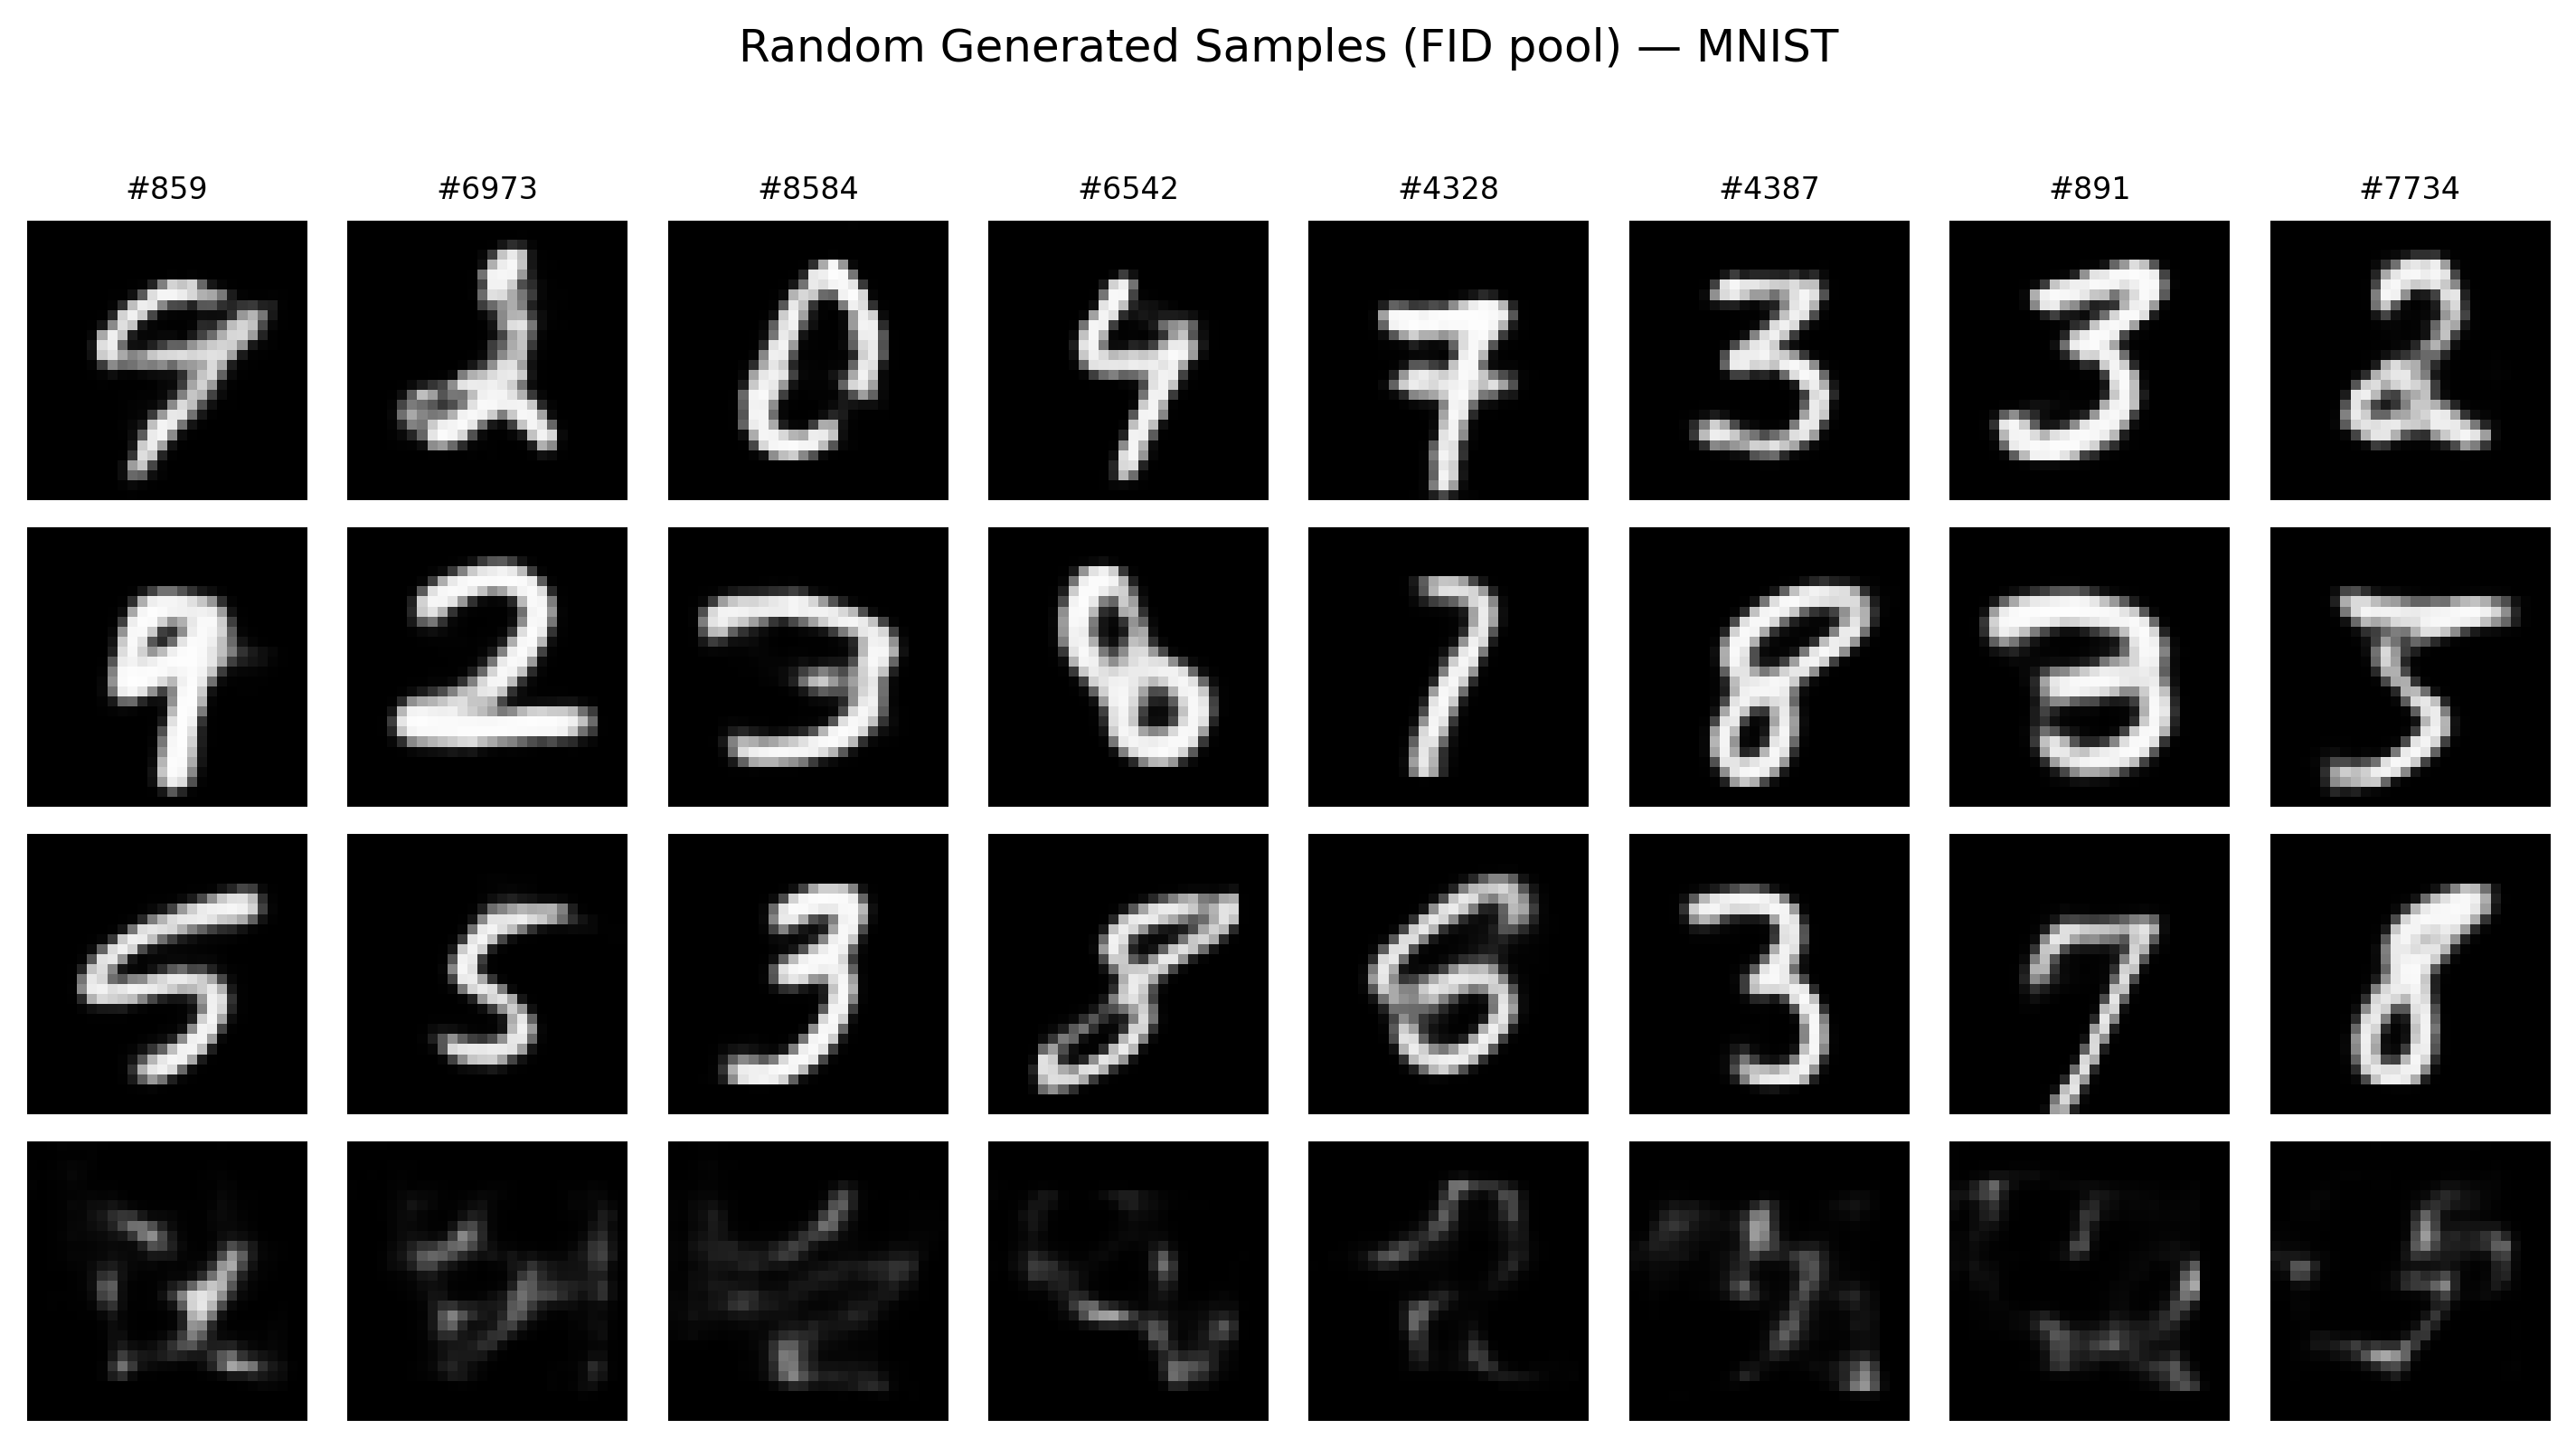
\includegraphics[width=\linewidth]{fig15_fid_samples_mnist.png}
    \caption{MNIST}
\end{subfigure}
\hfill
\begin{subfigure}{0.49\linewidth}
    \centering
    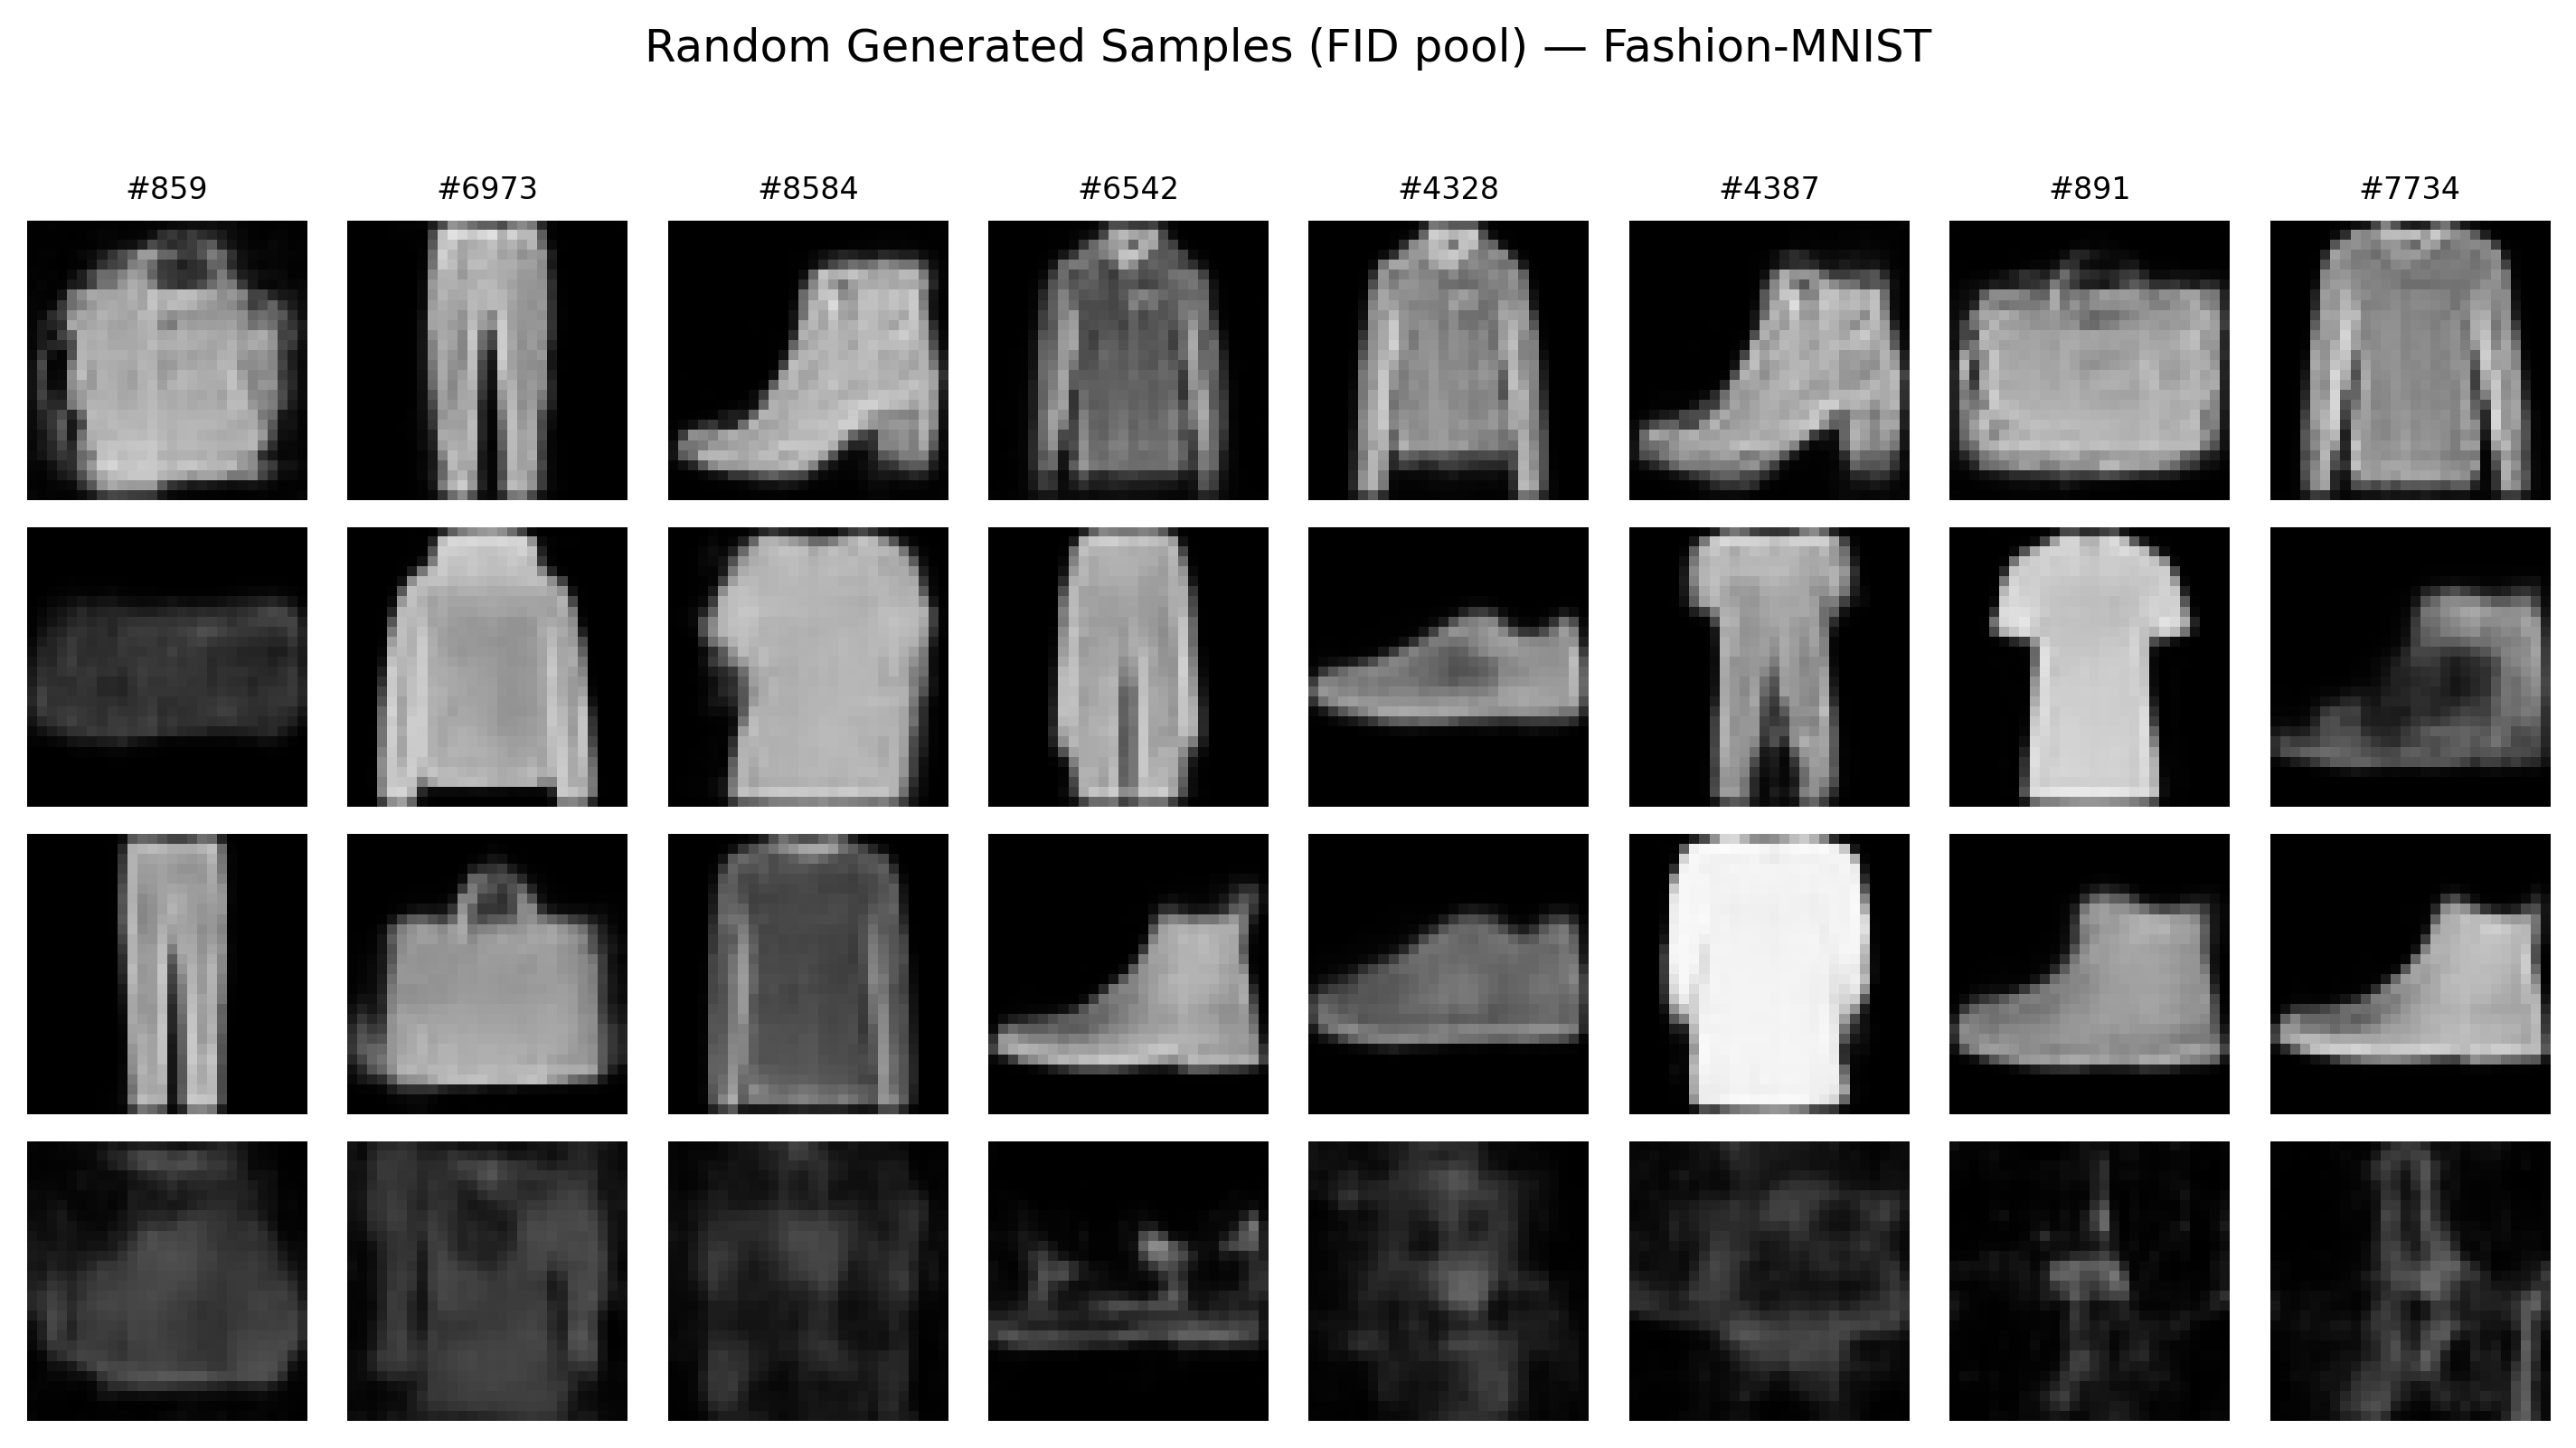
\includegraphics[width=\linewidth]{fig15_fid_samples_fashion_mnist.png}
    \caption{Fashion-MNIST}
\end{subfigure}
\caption{Random generated samples from the FID folders. These samples help interpret the gap between reconstruction quality and prior sample quality.}
\label{fig:fid-samples}
\end{figure}

\section{Discussion}

\paragraph{Why does the method work?}
The empirical pattern suggests that three factors reinforce each other. First, the hypersphere removes radial degrees of freedom and encourages representations to encode class identity directionally. Second, learnable class priors provide explicit anchors for each label. Third, MMD aligns distributions rather than individual points, allowing within-class variability around each prior. The Spherical Cauchy prior appears to offer a useful balance: it is concentrated enough to support class structure, but heavy-tailed enough to avoid the overly sharp behavior observed in some vMF variants.

Another way to view the method is as a distributional alternative to a classification head. A classifier would push features toward decision boundaries that are optimized for label prediction, but it would not directly define a generative prior. CS-WAE instead shapes the latent distribution itself. This is weaker than a classifier for pure accuracy, but stronger for generative use because sampling and clustering share the same latent geometry.

\paragraph{What should be claimed?}
The strongest defensible claim is that CS-WAE is a label-guided generative representation model with strong clustering behavior. It should not be presented as fully unsupervised clustering, because training uses labels. It also should not be presented as uniformly best for generation, because VaDE has lower FID on Fashion-MNIST. A precise claim is more powerful: CS-WAE substantially improves clustering under a simple K-means evaluation while maintaining competitive sample quality, and its ablations show that supervised MMD, spherical geometry, and Spherical Cauchy priors are all important.

\paragraph{Limitations.}
The current study has four limitations. First, baseline comparisons are single-seed, whereas the main CS-WAE table uses three seeds. Second, the MNIST ablation table uses an older training path, so the absolute MNIST ablation baseline should not be mixed with the main multi-seed number. Third, the experiments use only grayscale $28\times28$ datasets; larger and more complex datasets such as CIFAR-10, STL-10, or CelebA would test scalability. Fourth, the supervised MMD term assumes labels are available. A future semi-supervised variant could use labeled anchors plus unlabeled data, or replace class labels with pseudo-labels updated during training.

\paragraph{Practical implications.}
The current results suggest a practical recipe for tasks where labels exist during training but one still wants a generative latent space: do not treat reconstruction, clustering, and sampling as separate objectives bolted together at the end. Instead, design the latent prior so that class structure is part of the generative model. This is relevant for representation learning, controllable generation, and class-conditional data exploration on small or medium image datasets.

\section{Conclusion}

We presented CS-WAE, a class-structured Spherical Cauchy Wasserstein auto-encoder for label-guided generative clustering. The model combines hyperspherical latent geometry, learnable class priors, Spherical Cauchy reparameterization, and dual MMD regularization. Experiments on MNIST and Fashion-MNIST show strong clustering performance relative to VAE, VaDE, and WAE-MMD baselines, with ablations demonstrating that the supervised MMD term and spherical latent geometry are essential. More broadly, the results support the view that generative representation learning benefits from matching the geometry of the latent space to the intended downstream structure. For class-aware visual representation learning, the combination of spherical priors and distribution-level class alignment is a simple and effective design.

\bibliographystyle{plainnat}
\bibliography{references}

\appendix

\section{Additional Experimental Details}

\paragraph{Architecture.}
The encoder consists of three convolutional blocks followed by a fully connected layer. It outputs an unnormalized direction vector and a scalar radius parameter. The decoder maps the latent vector through a fully connected block and three transposed convolutional layers with a final sigmoid output. The latent dimension is 32.

\paragraph{Optimization.}
All experiments use Adam with learning rate $10^{-3}$, batch size 128, 50 epochs, gradient clipping with maximum norm 1.0, and StepLR with step 30 and multiplicative decay 0.5. The supervised and unsupervised MMD weights are linearly annealed over 20 epochs to 20 and 50, respectively.

\paragraph{Reconstruction metrics.}
The full implementation computes SSIM, PSNR, and LPIPS on the test set. The main paper reports clustering and FID to keep the core narrative focused. Reconstruction metrics are available in the repository outputs.

\section{Reproducibility Notes}

The reported artifacts were generated by the repository pipeline. Main CS-WAE runs store per-seed metrics in \texttt{runs/<dataset>/seed\_\{0,1,2\}/metrics.json}; aggregate metrics are stored in \texttt{runs/<dataset>/aggregated\_metrics.json}. Baseline results are stored in \texttt{runs/<dataset>/baselines/seed\_0/comparison\_results.csv}. Ablation results are stored in \texttt{runs/<dataset>/ablation\_*/ablation\_results.csv}.

\section{Recommended Next Experiments}

The most important next step is to run all baselines over the same three seeds as CS-WAE. The second is to rerun MNIST ablations with the aligned code path. The third is to evaluate on at least one higher-complexity dataset. These additions would make the empirical section substantially stronger for a competitive conference submission.

\end{document}
